
\documentclass[
tikz,
11pt, % The default document font size, options: 10pt, 11pt, 12pt
oneside, % Two side (alternating margins) for binding by default, uncomment to switch to one side
english, % ngerman for German
singlespacing, % Single line spacing, alternatives: onehalfspacing or doublespacing
%draft, % Uncomment to enable draft mode (no pictures, no links, overfull hboxes indicated)
%nolistspacing, % If the document is onehalfspacing or doublespacing, uncomment this to set spacing in lists to single
%liststotoc, % Uncomment to add the list of figures/tables/etc to the table of contents
%toctotoc, % Uncomment to add the main table of contents to the table of contents
%parskip, % Uncomment to add space between paragraphs
%nohyperref, % Uncomment to not load the hyperref package
headsepline, % Uncomment to get a line under the header
%chapterinoneline, % Uncomment to place the chapter title next to the number on one line
%consistentlayout, % Uncomment to change the layout of the declaration, abstract and acknowledgements pages to match the default layout
]{MastersDoctoralThesisV2} % The class file specifying the document structure

\usepackage[utf8]{inputenc} % Required for inputting international characters
\usepackage[T1]{fontenc} % Output font encoding for international characters
\usepackage{todonotes}
\usepackage{mathpazo} % Use the Palatino font by default
\usepackage{adjustbox} % Resize table
\usepackage[backend=bibtex,style=authoryear,natbib=true]{biblatex} % Use the bibtex backend with the authoryear citation style (which resembles APA)

\addbibresource{thesis.bib} % The filename of the bibliography
\usepackage{float}
\usepackage{graphicx}
\usepackage{rotating}
\usepackage[autostyle=true]{csquotes} % Required to generate language-dependent quotes in the bibliography
\usepackage{glossaries}
\usepackage[T1]{fontenc}
\usepackage{comment}
\makeglossaries
\loadglsentries{glossary}
\usetikzlibrary{fit,positioning}


\title{Statistical analysis of negative selection using pangenomics data models.
 Analisi statistiche per detectare la selezione negativa usando dati pangenomici.}

%Analisi statistiche per detectare la selezione negativa usando dati pangenomici.

\author{Flavia Villani }
\date{24 May 2020}



\begin{document}

\begin{titlepage}
\centering
{\scshape\large\normalfont\bfseries Università degli Studi di Napoli Federico II \par}
 \vspace{0.7cm} 
 
\includegraphics[width=0.25\textwidth]{fig/logo.png}
 \par
 \vspace{0.5cm}
\hspace{2cm}
{\scshape\large\normalfont Dipartimento di Medicina Molecolare e Biotecnologie Mediche

Area Didattica di Scienze Matematiche Fisiche e Naturali
 \par}
 \vspace{0.5cm}
{\scshape\large\normalfont Corso di Laurea Magistrale in Biotecnologie Mediche
 \par}
 \vspace{0.5cm} 
{\scshape\large\normalfont Tesi sperimentale in Genetica Medica
 \par}
  \vspace{0.8cm}
{\scshape\large\normalfont\bfseries\textit Statistical analysis of negative selection using pangenomics data models 
 \par}
  \vspace{0.8cm}
{\scshape\large\normalfont\bfseries  Analisi statistiche per detectare la selezione negativa usando dati pangenomici
 \par} 
\vspace{2cm} 
\begin{minipage}{0.45\textwidth}
{\scshape\normalfont\large\bfseries Relatore interna:}\\
{\scshape\normalfont\large Dott.ssa Gabriella De Vita} \\ 
{\scshape\normalfont\large\bfseries Relatrice esterna:} \\
{\scshape\normalfont\large Dott.ssa Vincenza Colonna}\\
\end{minipage}
\hspace{2.5cm}
\begin{minipage}{0.25\textwidth}
{\scshape\normalfont\large\bfseries Candidato:}\\
 {\scshape\normalfont\large Flavia Villani \\
 Matricola N79001438} 
\end{minipage}

\vfill
\centering
\vspace{0.48cm} 
{\scshape\Large\normalfont A.A. 2019/2020}

\end{titlepage}
%\maketitle
%----------------------------------------------------------------------------------------
%	LIST OF CONTENTS/FIGURES/TABLES PAGES
%----------------------------------------------------------------------------------------

\tableofcontents % Prints the main table of contents

%\listoffigures % Prints the list of figures

%\listoftables % Prints the list of tables


%----------------------------------------------------------------------------------------
\chapter{Sommario / Abstract(1 pagina)}
 
Studies of genomic selection typically assume a single linear reference genome. However,
structural and complex variation can render these simplified models inapplicable. To address this
limitation, in my thesis, I am working to implement a software library for the statistical analysis of
negative selection using pangenomic data models. Typically represented in the Graphical Fragment
Assembly (GFA) format, these models can represent whole genome alignments in a compact
graphical structure. Because they embed the linear genomes from which they are constructed, we
can choose a particular reference genome and project the variants (which appear as bubbles in the
graph) back into any reference frame. Thus far, I have focused on algorithms for bubble detection
that allow us to generate Variant Call Format (VCF) files from graphs. We can use this projection to
drive standard population genetic analyses, or eventually as a mechanism to communicate results
that we obtain from pangenome graph based population genetic analyses which I am designing.

\chapter{Introduction/(5-10 pagine)}

\section {Graphical Fragment Assembly (GFA) Format Specification }
Format 
\section {Variant Call Format (VCF) }
Format

\section{Simulation }
MP
F-test 
\section{Application}

\chapter{Results of the Research Group (5-10 pagine) }
Descrive il progetto di ricerca di cui fa parte l’attività sperimentale svolta dal candidato. Vanno qui riportati i risultati ottenuti dal gruppo di ricerca in precedenza e/o in contemporanea rispetto all’attività svolta dal candidato che siano rilevanti per l’argomento della tesi. Nel caso in cui il candidato abbia svolto, nell’ambito del gruppo di appartenenza, un progetto di ricerca nuovo e autonomo, questa sezione può essere eliminata. In questa sezione è richiesto l’uso di illustrazioni.
 
\chapter{Aims of the thesis/(1-2 pagine)}
The aims of the thesis is how drive standard population genetic analyses of negative selection using pangenomic data models. Typically represented in the Graphical Fragment Assembly (GFA) format, these models can represent whole genome alignments in a compact graphical structure. Thus far, I have focused on algorithms for bubble detection that allow us to generate Variant Call Format(VCF) files from graphs. 


\chapter{Results achieved by the Candidate(5-20 pagine)}
%%%%%%%%%%%%%%%%%%%%%%%%%%%%%%%%%%%%%%%%%%%%%%%%%%%%%%%%%%%
%  Section 
%%%%%%%%%%%%%%%%%%%%%%%%%%%%%%%%%%%%%%%%%%%%%%%%%%%%%%%%%%%
\section{From Graphical Fragment Assembly (GFA) format to VCF}
Data consists of GFA format from simulation of genomic sequences. From a GFA I'm obtained VCF. 

DNA sequence graphs represented by (Figure \ref{fig:x.pdf}) have two strands, we need a more precise way of addressing elements in the graph than nodes, which implicitly represent both strands. The handle, allows us to refer to one strand of a single node, which is the smallest addressable unit in a variation graph. Nodes have numeric identifiers (or IDs), and associated sequences. Edges link two handles. Paths are a series of steps which link a path identifier and a handle.
\cite({garrison2020}). 

\begin{comment}
{\small
\begin{table}
\caption{Element of GFA}
\label{tab:stats_variantcalling}
\centering
\begin{adjustbox}{width=1\textwidth}
\begin{tabular}{1 1 1 1 1 1 1}
\toprule
\tabhead{} & \tabhead{} & \tabhead{} & \tabhead{}\\
\midrule
Handle & an oriented traversal of a node (an opaque 64-bit identifier) \\
ID & a node identifier\\
Edge & a pair of handle, where the edge is directed from the first member of the pair to the second \\
Path_handle & a reference to a path \\
Step_handle & a reference to a single step of a path on one node traversal \\
\bottomrule\\
\end{tabular}
\end{adjustbox}
\end{table}
} 
\end{comment}
I obtained the element of the VCF from GFA:
\begin{itemize}
    \item CHROM: name of the path in the GFA
    \item POS: lengh of sequence in that position 
    \item REF: path of reference that I chose
    \item ALT: sequence that not present in the ref, alt present in the bubble
    \item TYPE: SNV, INDEL, INSERTION 
\end{itemize}

 

\begin{figure}[H]
\centering
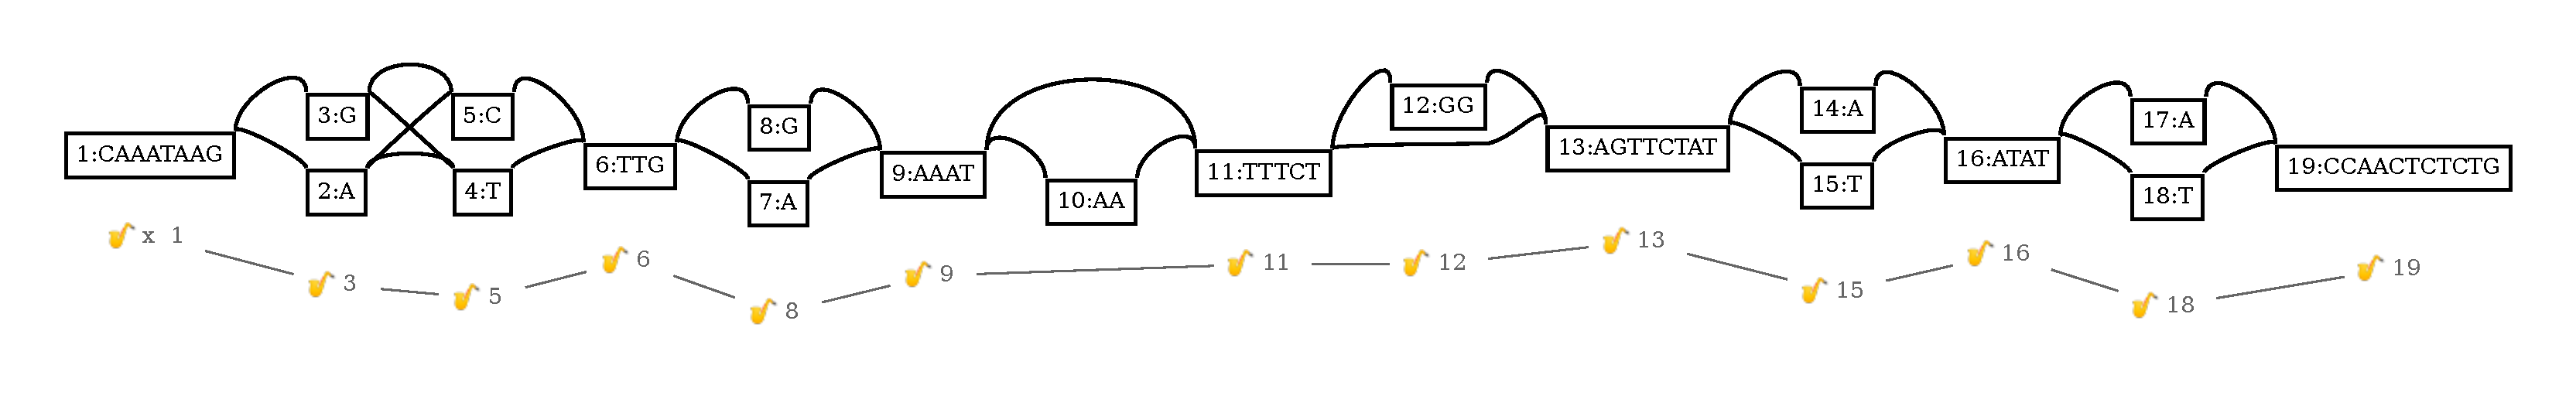
\includegraphics[width=1.10\textwidth]{fig/x.pdf}
\decoRule
\caption{\textbf{Fig:} node id, sequence, insertion, deletion \textbf}
\label{fig:x.pdf}
\end{figure}









\begin{comment}
    \begin{tikzpicture}[
    node distance = 7mm and -3mm,
every node/.style = {draw=black, rounded corners, fill=gray!30, 
                     minimum width=2cm, minimum height=0.5cm,
                     align=center},
every path/.style = {draw, -latex}
                        ]
\node (start) {GFA-->VCF};
\node (start) {GFA-->ODGI-->VCF}
%
\node (y1) [below  left=of start]       {Y1}; 
\node (y2) [below right=of y1.east]     {Y2};
\node (y3) [below right=of y2.east]     {Y3};
%
\node (x1) [right=12mm of y3.east |- y1]{X1};
\node (x2) [right=12mm of y3.east |- y2]{X2};
\node (x3) [right=12mm of y3.east]      {X2};
%
\node (end) [below=21mm of y2 |- y3]    {END};
%
\node [dashed, fill=none, fit=(x1) (x3)] {};
%%
\draw   (start) -| (y1);
\draw   (start) -- (y2);
\draw   (start) -| (y3);
%
\draw   (x1) edge (y1)
        (x2) edge (y2)
        (x3)  to  (y3);
%
    \begin{scope}[densely dashed]
\draw   (y1) |- ([shift={(-5mm,9mm)}] end.north) -- ([xshift=-5mm] end.north);
\draw   (y2) -- (end);
\draw   (y3) |- ([shift={( 5mm,9mm)}] end.north) -- ([xshift= 5mm] end.north);
%
\draw   (y1 |- y2) -- (y2);
\draw[transform canvas={yshift= 1mm}]  (y1 |- y3) -- (y3);
\draw[transform canvas={yshift=-1mm}]  (y2 |- y3) -- (y3);
    \end{scope}
    \end{tikzpicture}
\end{comment}




















\begingroup 
\obeylines
\input{q.gfa}%
\endgroup%



%%%%%%%%%%%%%%%%%%%%%%%%%%%%%%%%%%%%%%%%%%%%%%%%%%%%%%%%%%%
%  Section 
%%%%%%%%%%%%%%%%%%%%%%%%%%%%%%%%%%%%%%%%%%%%%%%%%%%%%%%%%%%

\section{Identification of euploid samples for genetic analyses}
\todo{vedere note per articolo da citare}
In half of pregnancies in the first trimester the cause of PL are large chromosomal aneuploidies, such as trisomies or deletions of large chromosomal chunks (\cite{goddijn2000genetic}, \cite{zhang2009genetic}). With this project we want to focus on cases in which the embryo is euploid when analyzed with current diagnostic techniques i.e. comparative genomic hybridization (arrayCGH). Hence, samples were screened for chromosomal aneuploidies prior to whole-genome sequencing. This task was performed before my thesis work started, nevertheless I am describing it here because of its importance. \\

In 44 samples when screened for maternal contamination 11.4\% drops off the analysis, due to technical challenges during sample collection. A first round of detection of aneuploidies on chromosomes 13, 15, 16, 18, 21, 22, X, and Y through Short Tandem Repeats analysis discarded 47.7\% of samples. These types of repeats (tetra- or penta-nucleotide) are often expected to be found in heterozygosis, therefore triploidies are assumed when three alleles are found at several markers along a chromosome (complete) or part of it (partial). Similarly, uniparental disomy for a targeted region or chromosome is assumed when only one parental allele is amplified. Subsequent analysis through array-CGH and \gls{copy number variation} detection form low-coverage sequencing discarded another 11.4\% of samples (Figure \ref{fig:pipelineOutcome}).

The most common aneuploidy in our data set is the trisomy of chromosome 22 (15.9\%), followed by trisomy of chromosome 16 (9\%) and 18 (4.5\%)(Figure \ref{fig:preseqOutcome}).

%Another step for choosing is detection of copy number variants through comparative genomic hybridization ) using an assay with 60k probes genome-wide distributed. Most of the aneuploidies are trisomy of chromosome 22 and more in recurrent miscarriage than miscarriage first 

Overall 29.5\% of samples were euploid (Figure \ref{fig:preseqOutcome}) and could proceed to whole-genome sequence analysis. By the time I started my thesis I had access to six samples for which sequence data was ready and available to be sequenced. 


\begin{figure}[H]
\centering
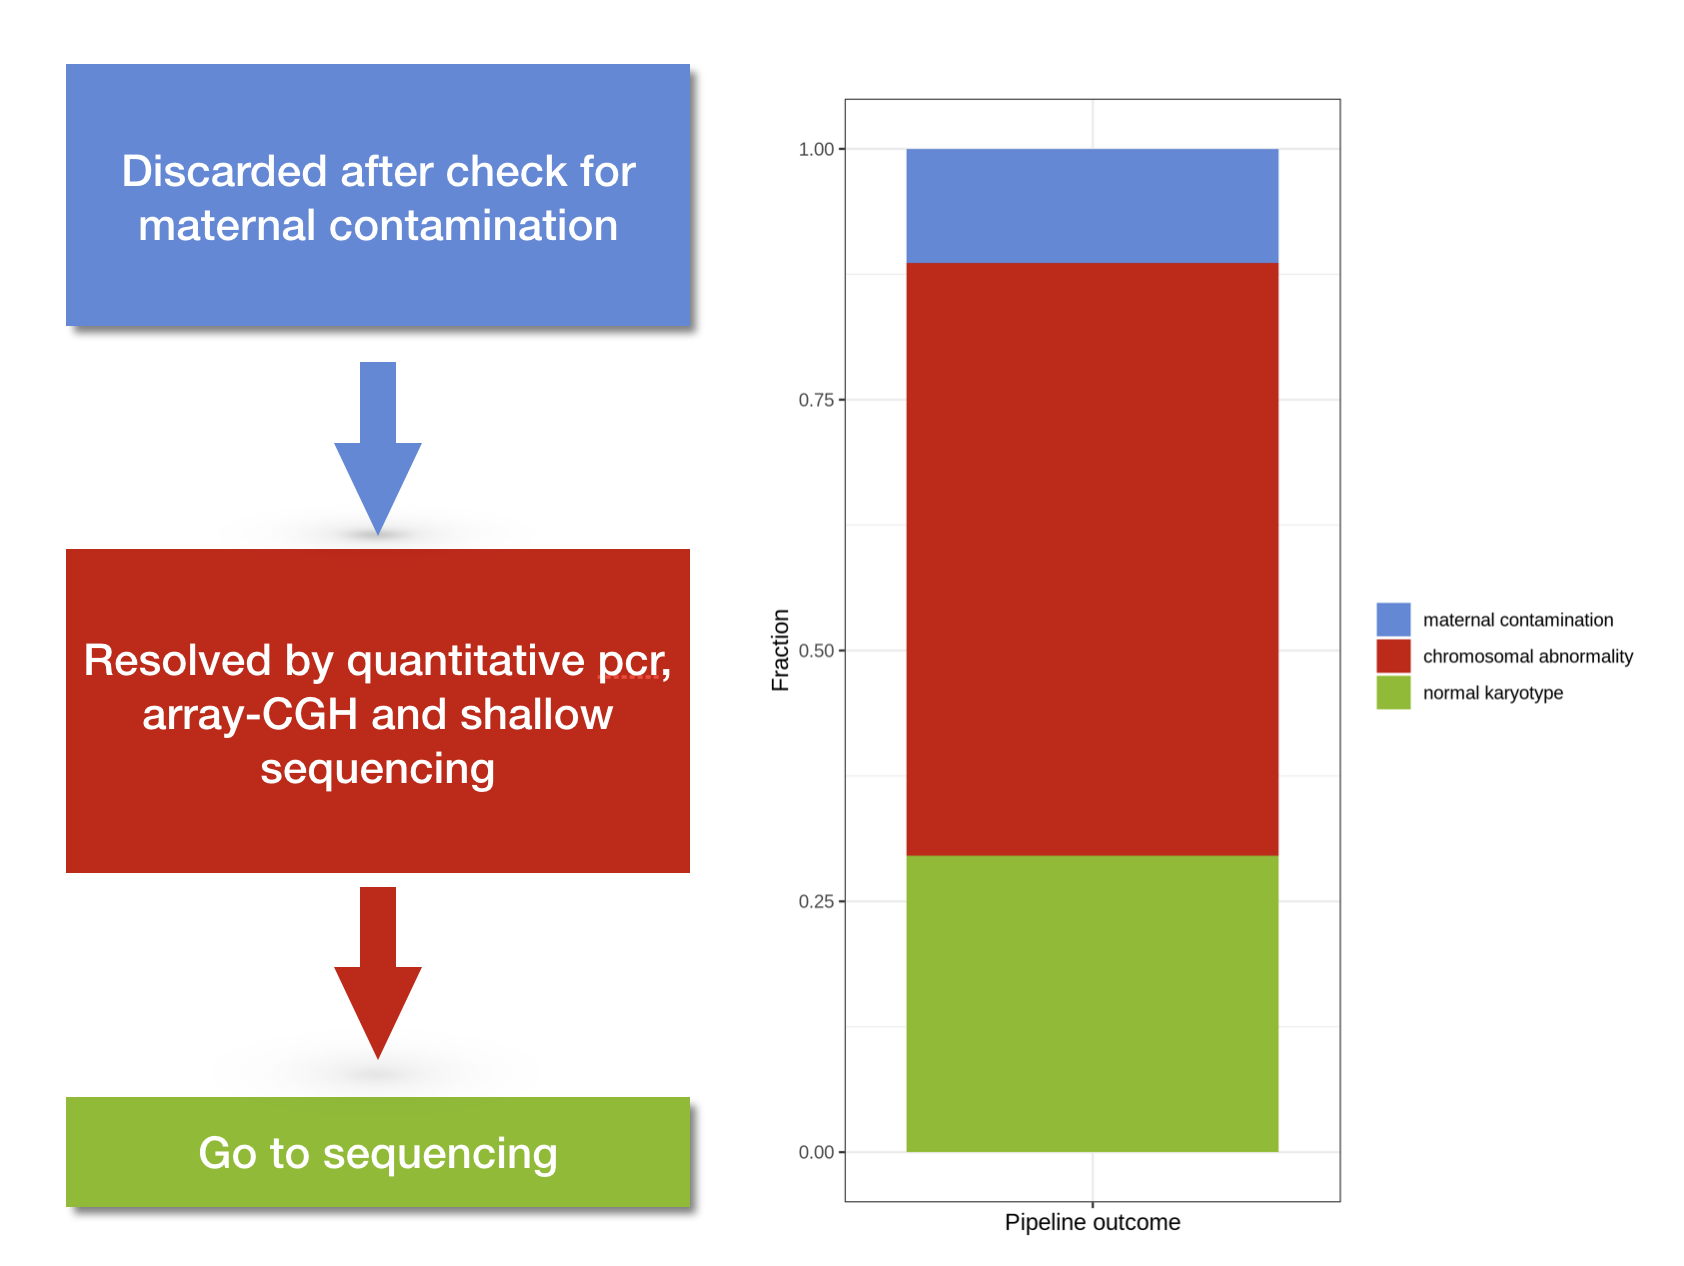
\includegraphics[width=0.85\textwidth]{fig/sampletocollectG.png}
\decoRule
\caption{\textbf{Pipeline outcome.} Percentage of samples that was discarded/go to sequencing }
\label{fig:pipelineOutcome}
\end{figure}

\begin{figure}[H]
\centering
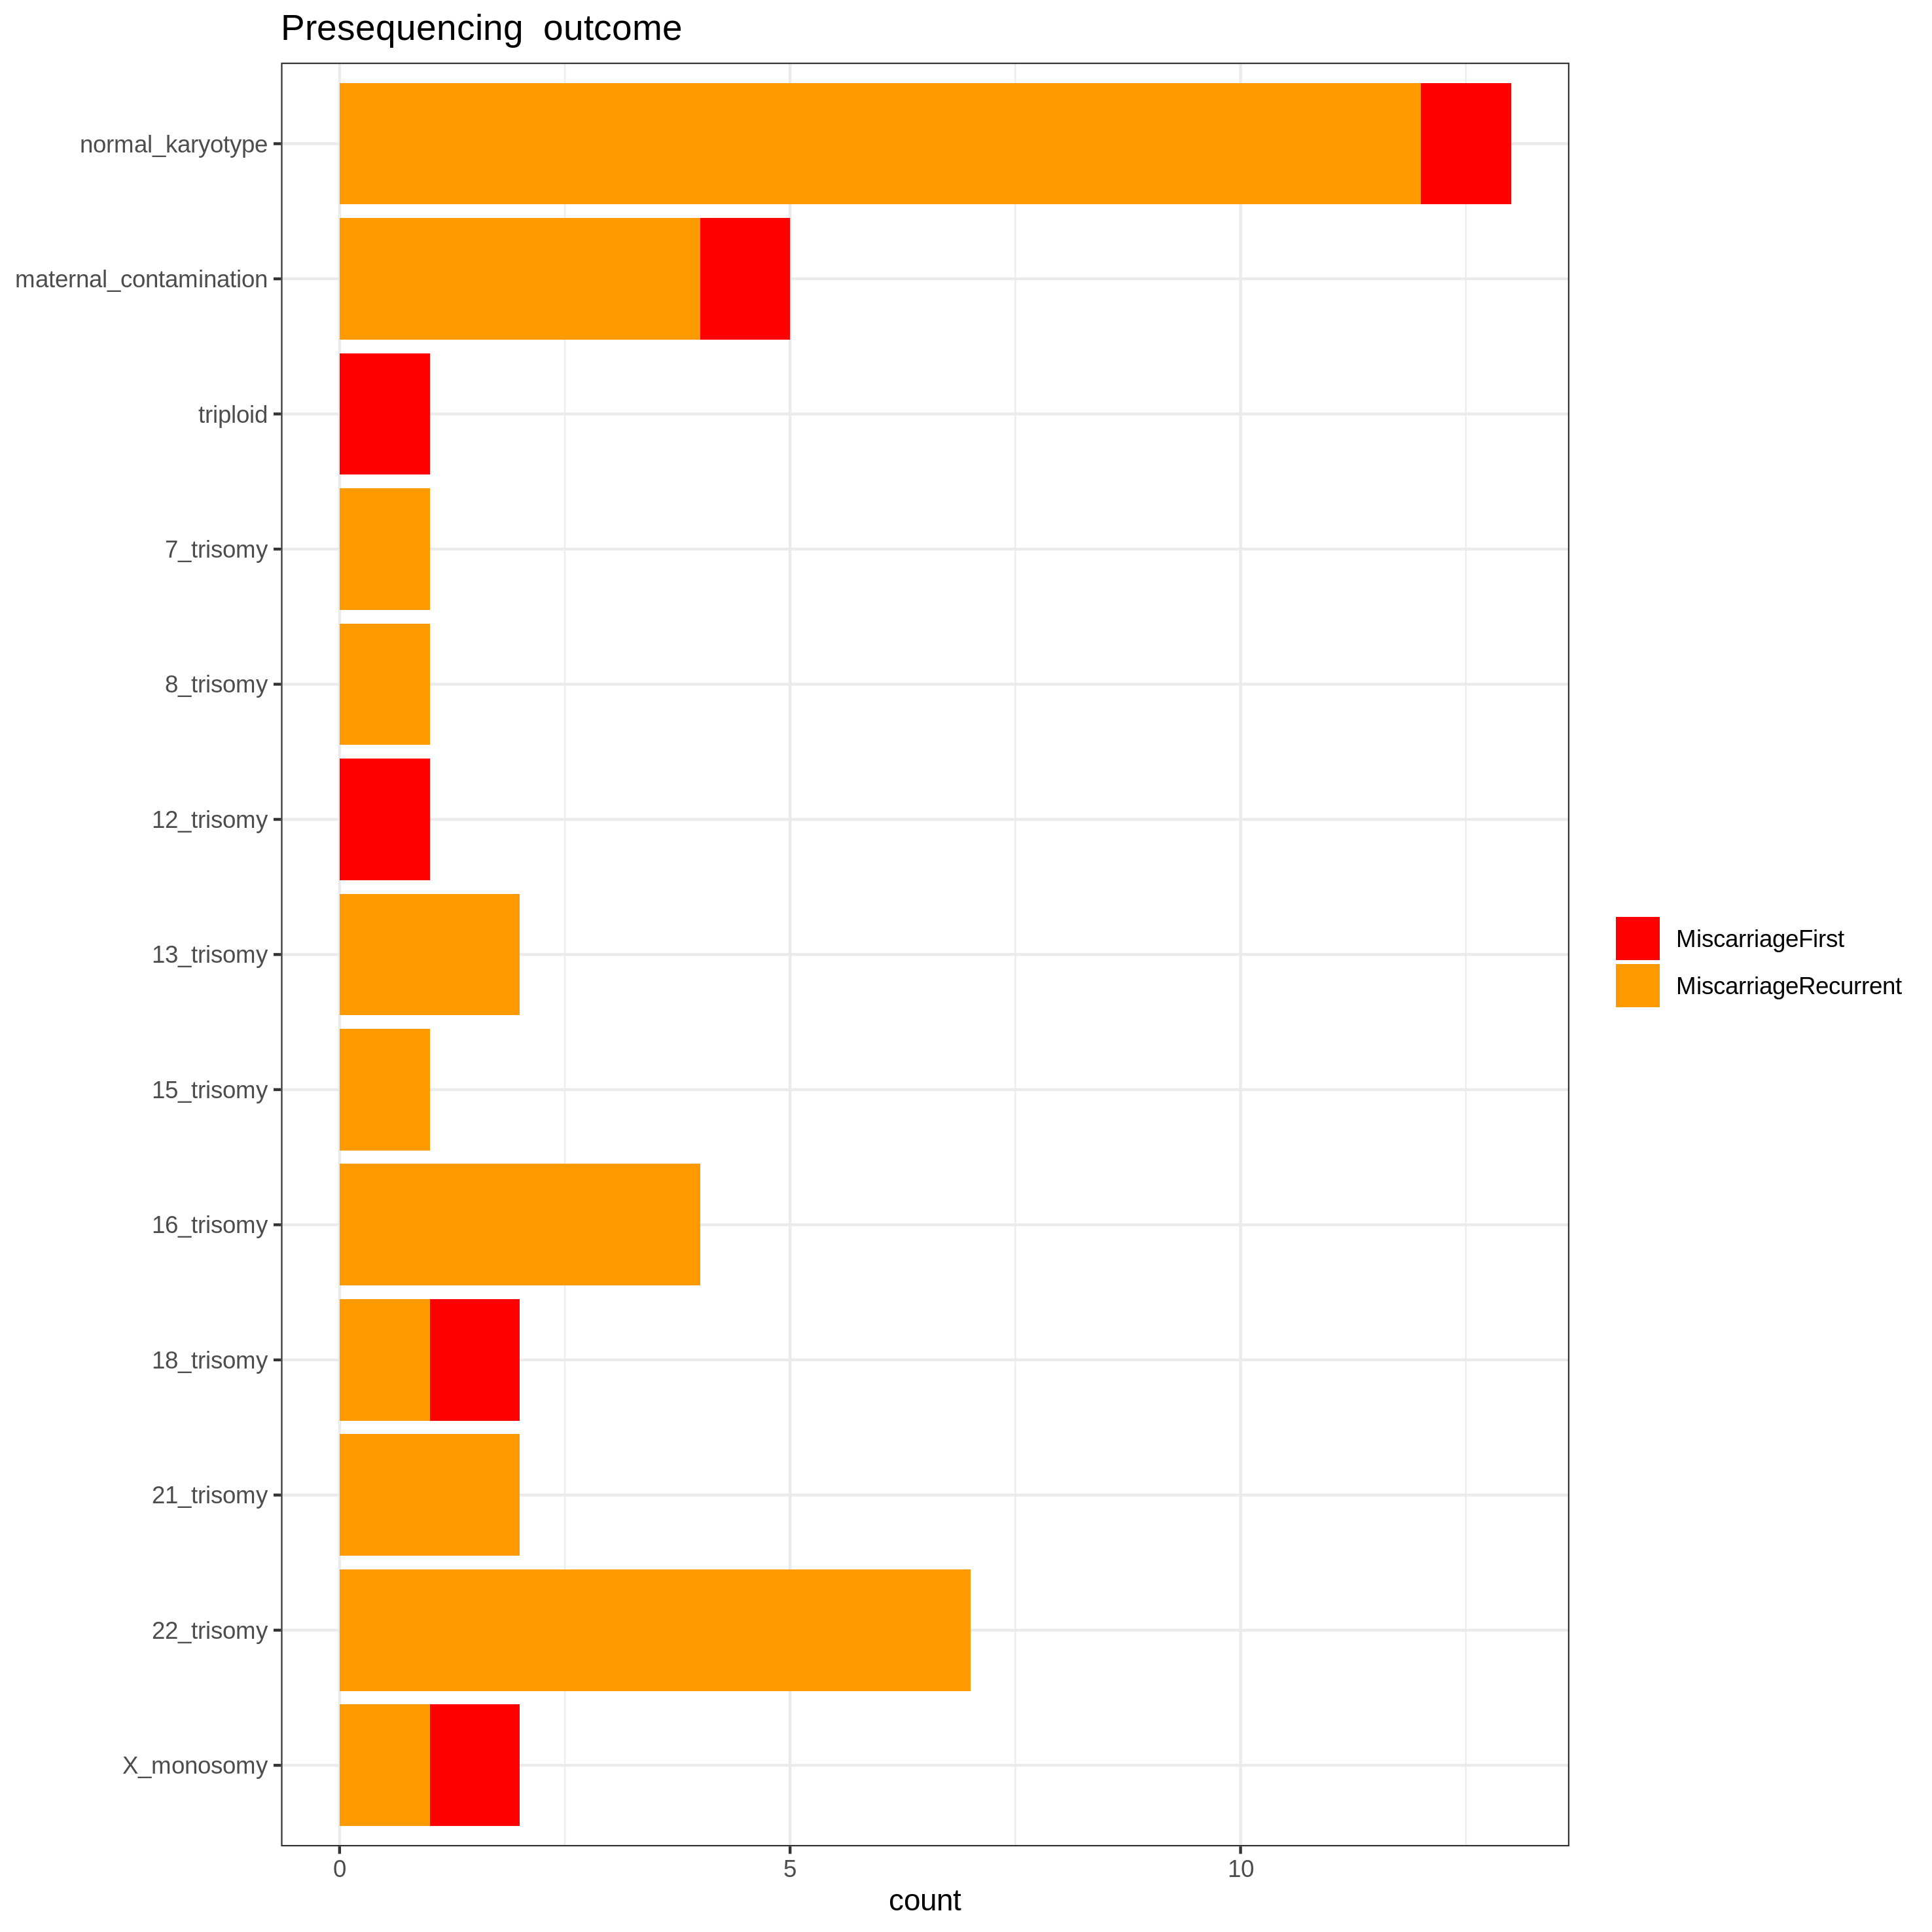
\includegraphics[width=0.8\textwidth]{fig/preseqOutcome.png}
\decoRule
\caption{\textbf{Number of aneuploidies on Samples.} 29.5\% of cases are diploid. The most common aneuploidies is a trisomy on chromosome 22 followed by trisomy on chromosome 16 and 18. 11.4\% was discarded for maternal contamination.}
\label{fig:preseqOutcome}
\end{figure}


%%%%%%%%%%%%%%%%%%%%%%%%%%%%%%%%%%%%%%%%%%%%%%%%%%%%%%%%%%%
%  Section 
%%%%%%%%%%%%%%%%%%%%%%%%%%%%%%%%%%%%%%%%%%%%%%%%%%%%%%%%%%%

\section{Analysis of whole-genome sequence of embryos from pregnancy loss}
\subsection{Pipeline for the identification of genetic variants}
The sequencing pipeline produces sequence data in the \gls{fastq} format that constitute the raw sequence data and can be used to perform the analysis from scratch and customized pipelines on \gls{high performance computing} machines. Figure \ref{fig:align-ref-vc} provides an overview of the pipeline used in this study.

I performed the \textbf{alignment} of the raw sequence data in form of \gls{reads} against the most recent version of the human reference Genome (GRChg38.p12, \cite{rosenbloom2015ucsc}) using \textsc{bwa-mem} (\cite{li2013aligning}) and \textsc{samtools} (\cite{li2009sequence}). The alignment produces files in the \gls{bam} format that provide information on the quality of the alignemnt and enable some quality controls. In our data set XX\% of reads were correctly aligned to the reference genome. The average \gls{coverage} is XXXX INSERIRE DATI DI STATISTICHE sul BAM.   
Before proceeding to the next step I used \textsc{sambamba} (\cite{tarasov2015sambamba}) to \textbf{refine} the data and remove PCR duplicates, i.e. reads and they came from the same DNA fragment that bias variant detection through increased homozygosity.

I used the refined bam file to perform \textbf{variant calling} using \textsc{freebayes} (\cite{garrison2012haplotype}) that produces data in the \gls{vcf} format. The variant calling is the process of identification of variants from sequence data, where variants are chunks of sequence that differ from the reference genome. Genetic variants are classified as single nucleotide variants (SNVs), small insertions and deletions (indels), and structural variants (SVs, large genomic rearrangements). In addition to call variants, the software specifies whether samples are homozygous or heterozygous (genotype) at the variable sites and the \gls{genotype likelihood}, i.e. the probability that the observed genotype is correct. 



%At this stage, for each samples in a specific format called BAM, with each BAM we are able to do a Variant Calling using another bioinformatics software called FREEBAYES developed by our collaborator Erik Garrison.

%This software, like the word says, calls the variants that differ from the reference genome and for variants we mean each base of genome that is not like in the reference genome. 
%Another positive thing is that the software can specify whether our samples are homozygous or heterozygous at those sites and for those alleles,  all supported by a likelihood score for each site.

The final step is a second round of \textbf{refining} that includes three steps. 
\begin{itemize}
    \item I used \textsc{vcffilter} (\cite{vcflib}) to filter variants for \gls{quality score}(QUAL)>20. The QUAL is an estimate of how likely it is to observe a call by chance, and a value of 20 corresponds to 1\% probability of having an incorrect genotype.
    \item I used \textsc{vt} (\cite{tan2015unified}) to do the normalization that consist of two parts: parsimony and left alignment. Parsimony is the representation of a variant in as few nucleotides as possible without reducing the length of any allele to 0. Left alignment is the shift of the start position of a variant to the left till it is no longer possible to do so (Figure \ref{fig:vtNorm}) (\cite{tan2015unified}).
    \item I used \textsc{vt} to deconstruct multiallelic variants in a VCF to allow for allelic comparisons between call sets (Figure \ref{fig:vtDecomp}) (\cite{tan2015unified}).
\end{itemize}

Overall, the variant calling identified on average 4.7M variant site \textit{per} sample. This number corresponds to the expectation in individuals of European ancestry( \cite{1000genome2015global}). The most represented class is single nucleotide variant (83.2\%) followed by insertions (6.85\% ) and deletions (6.84\%)(Figure \ref{fig:variantClass})(Table \ref{tab:variantClassMean}). \\


\begin{comment}
{\small
\begin{table}
\caption{Variant classes count}
\label{tab:stats_variantcalling}
\centering
\begin{adjustbox}{width=1\textwidth}
\begin{tabular}{1 1 1 1 1 1 1}
\toprule
\tabhead{ID} & \tabhead{SNV} & \tabhead{Deletion} & \tabhead{Insertion} & \tabhead{Indel} & \tabhead{Sequence alteration} & \tabhead{Substitution}   \\
\midrule
AS006 & 4,5M & 365k & 366k & 93k & 63k & 14k \\
AS054 & 4,6M & 379k & 378k & 98k & 68k & 16k \\
AS064 & 3,9M & 326k & 324k & 79k & 45k & 10k \\
AS074 & 3,9M & 331k & 331k & 82k & 49k & 10k \\
AS090 & 4,0M & 326k & 326k & 80k & 46k & 10k \\
AS094 & 3,8M & 325k & 323k & 78k & 45k & 10k \\
\bottomrule\\
\end{tabular}
\end{adjustbox}
\end{table}
}

{\small
\begin{table}
\caption{Mean of Variant classes in samples}
\label{tab:variantClassMean}
\centering
\begin{adjustbox}{width=1\textwidth}
\begin{tabular}{1 1 1 1 1 1}
\toprule
\tabhead{SNV} & \tabhead{Insertion} & \tabhead{Deletion} & \tabhead{Indel} & \tabhead{Sequence alteration} & \tabhead{Substitution}   \\
\midrule
0.8328 & 0.0685 & 0.0684 & 0.0170 & 0.0105 & 0.0024 	\\
\bottomrule\\
\end{tabular}
\end{adjustbox}
\end{table}
}

\end{comment}
\begin{figure}[H]
\centering
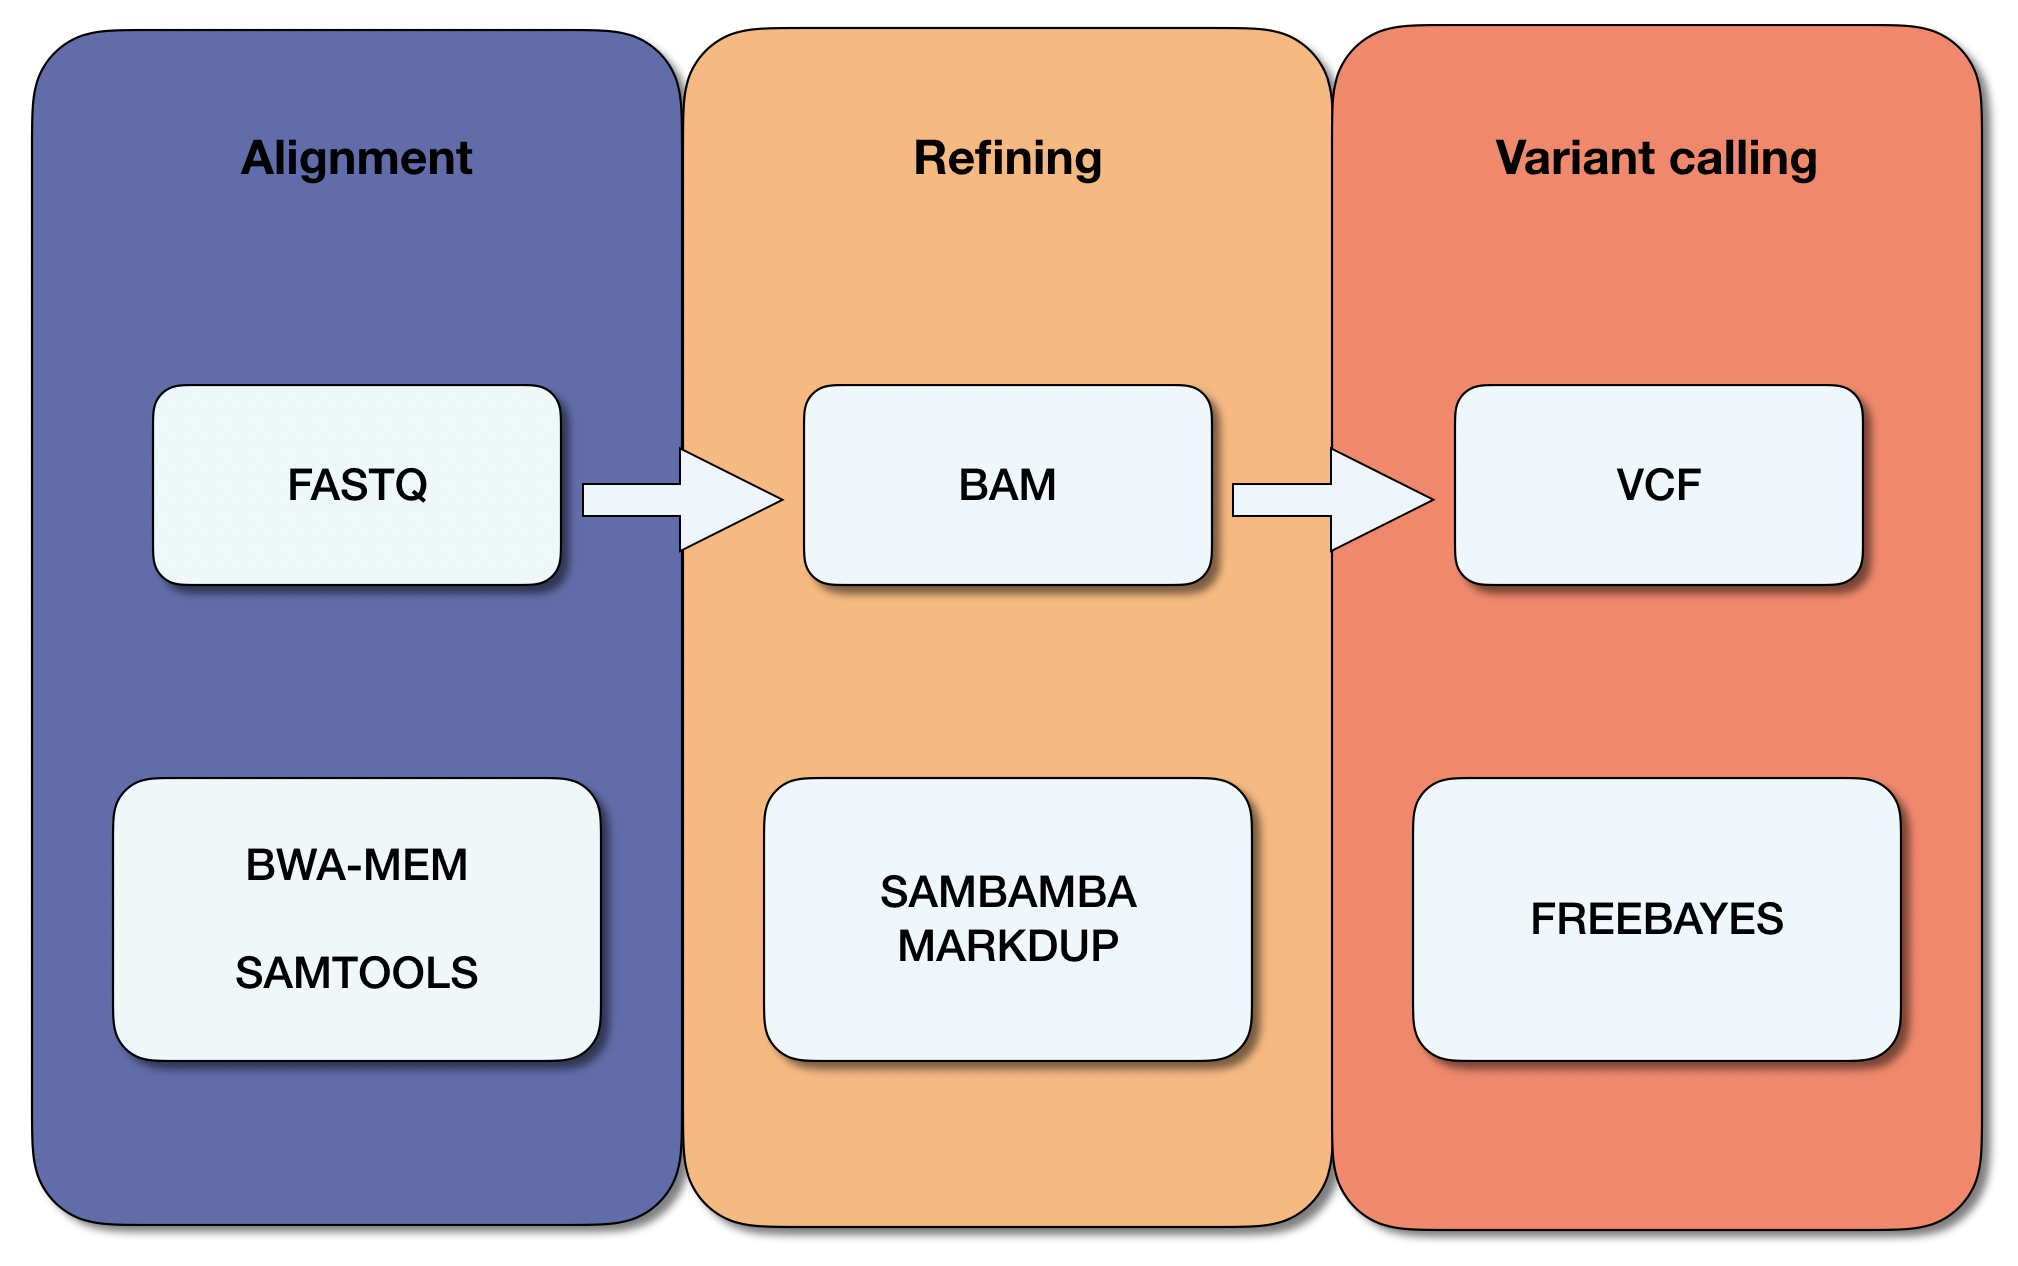
\includegraphics[width=0.65\textwidth]{fig/align-ref-vc.png}
\decoRule
\caption{\textbf{Pipeline.} From FASTQ to VCF.} 
\label{fig:align-ref-vc}
\end{figure}

\begin{figure}[H]
\centering
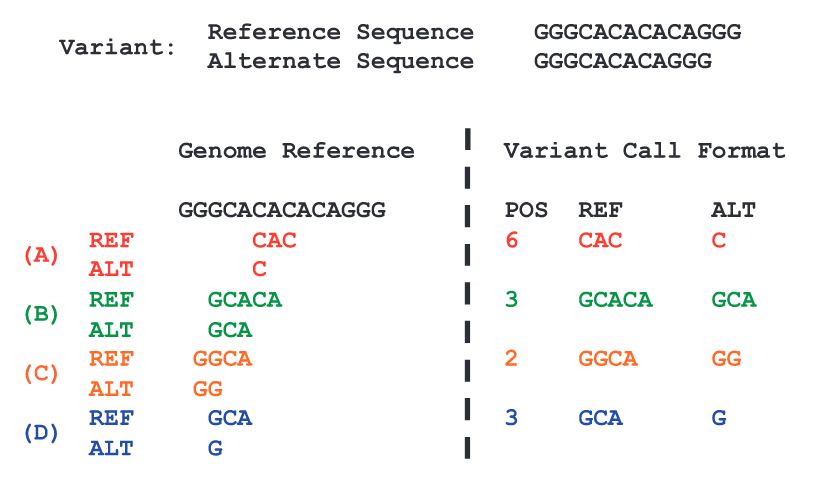
\includegraphics[width=0.65\textwidth]{fig/vtNormalizeTan.png}
\decoRule
\caption{\textbf{Example  of  VCF  entries  representing  the  same  variant.} \textit{ Adapted from \cite{tan2015unified}}. Left  panelaligns each allele to the reference genome, and the right panel represents thevariant in VCF. (A) is not left-aligned (B) is neither left-aligned nor parsimoni-ous, (C) is not parsimonious and (D) is normalized}
\label{fig:vtNorm}
\end{figure}

\begin{figure}[H]
\centering
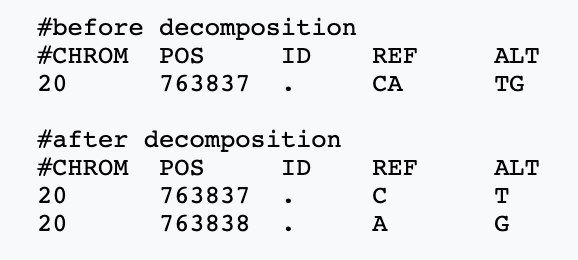
\includegraphics[width=0.5\textwidth]{fig/vtDecompose.png}
\decoRule
\caption{\textbf{Decomposes biallelic clumped variant} for allelic comparisons between call sets} \textit{ Adapted from \cite{tan2015unified}}. 
\label{fig:vtDecomp}
\end{figure}

\begin{figure}[H]
\centering
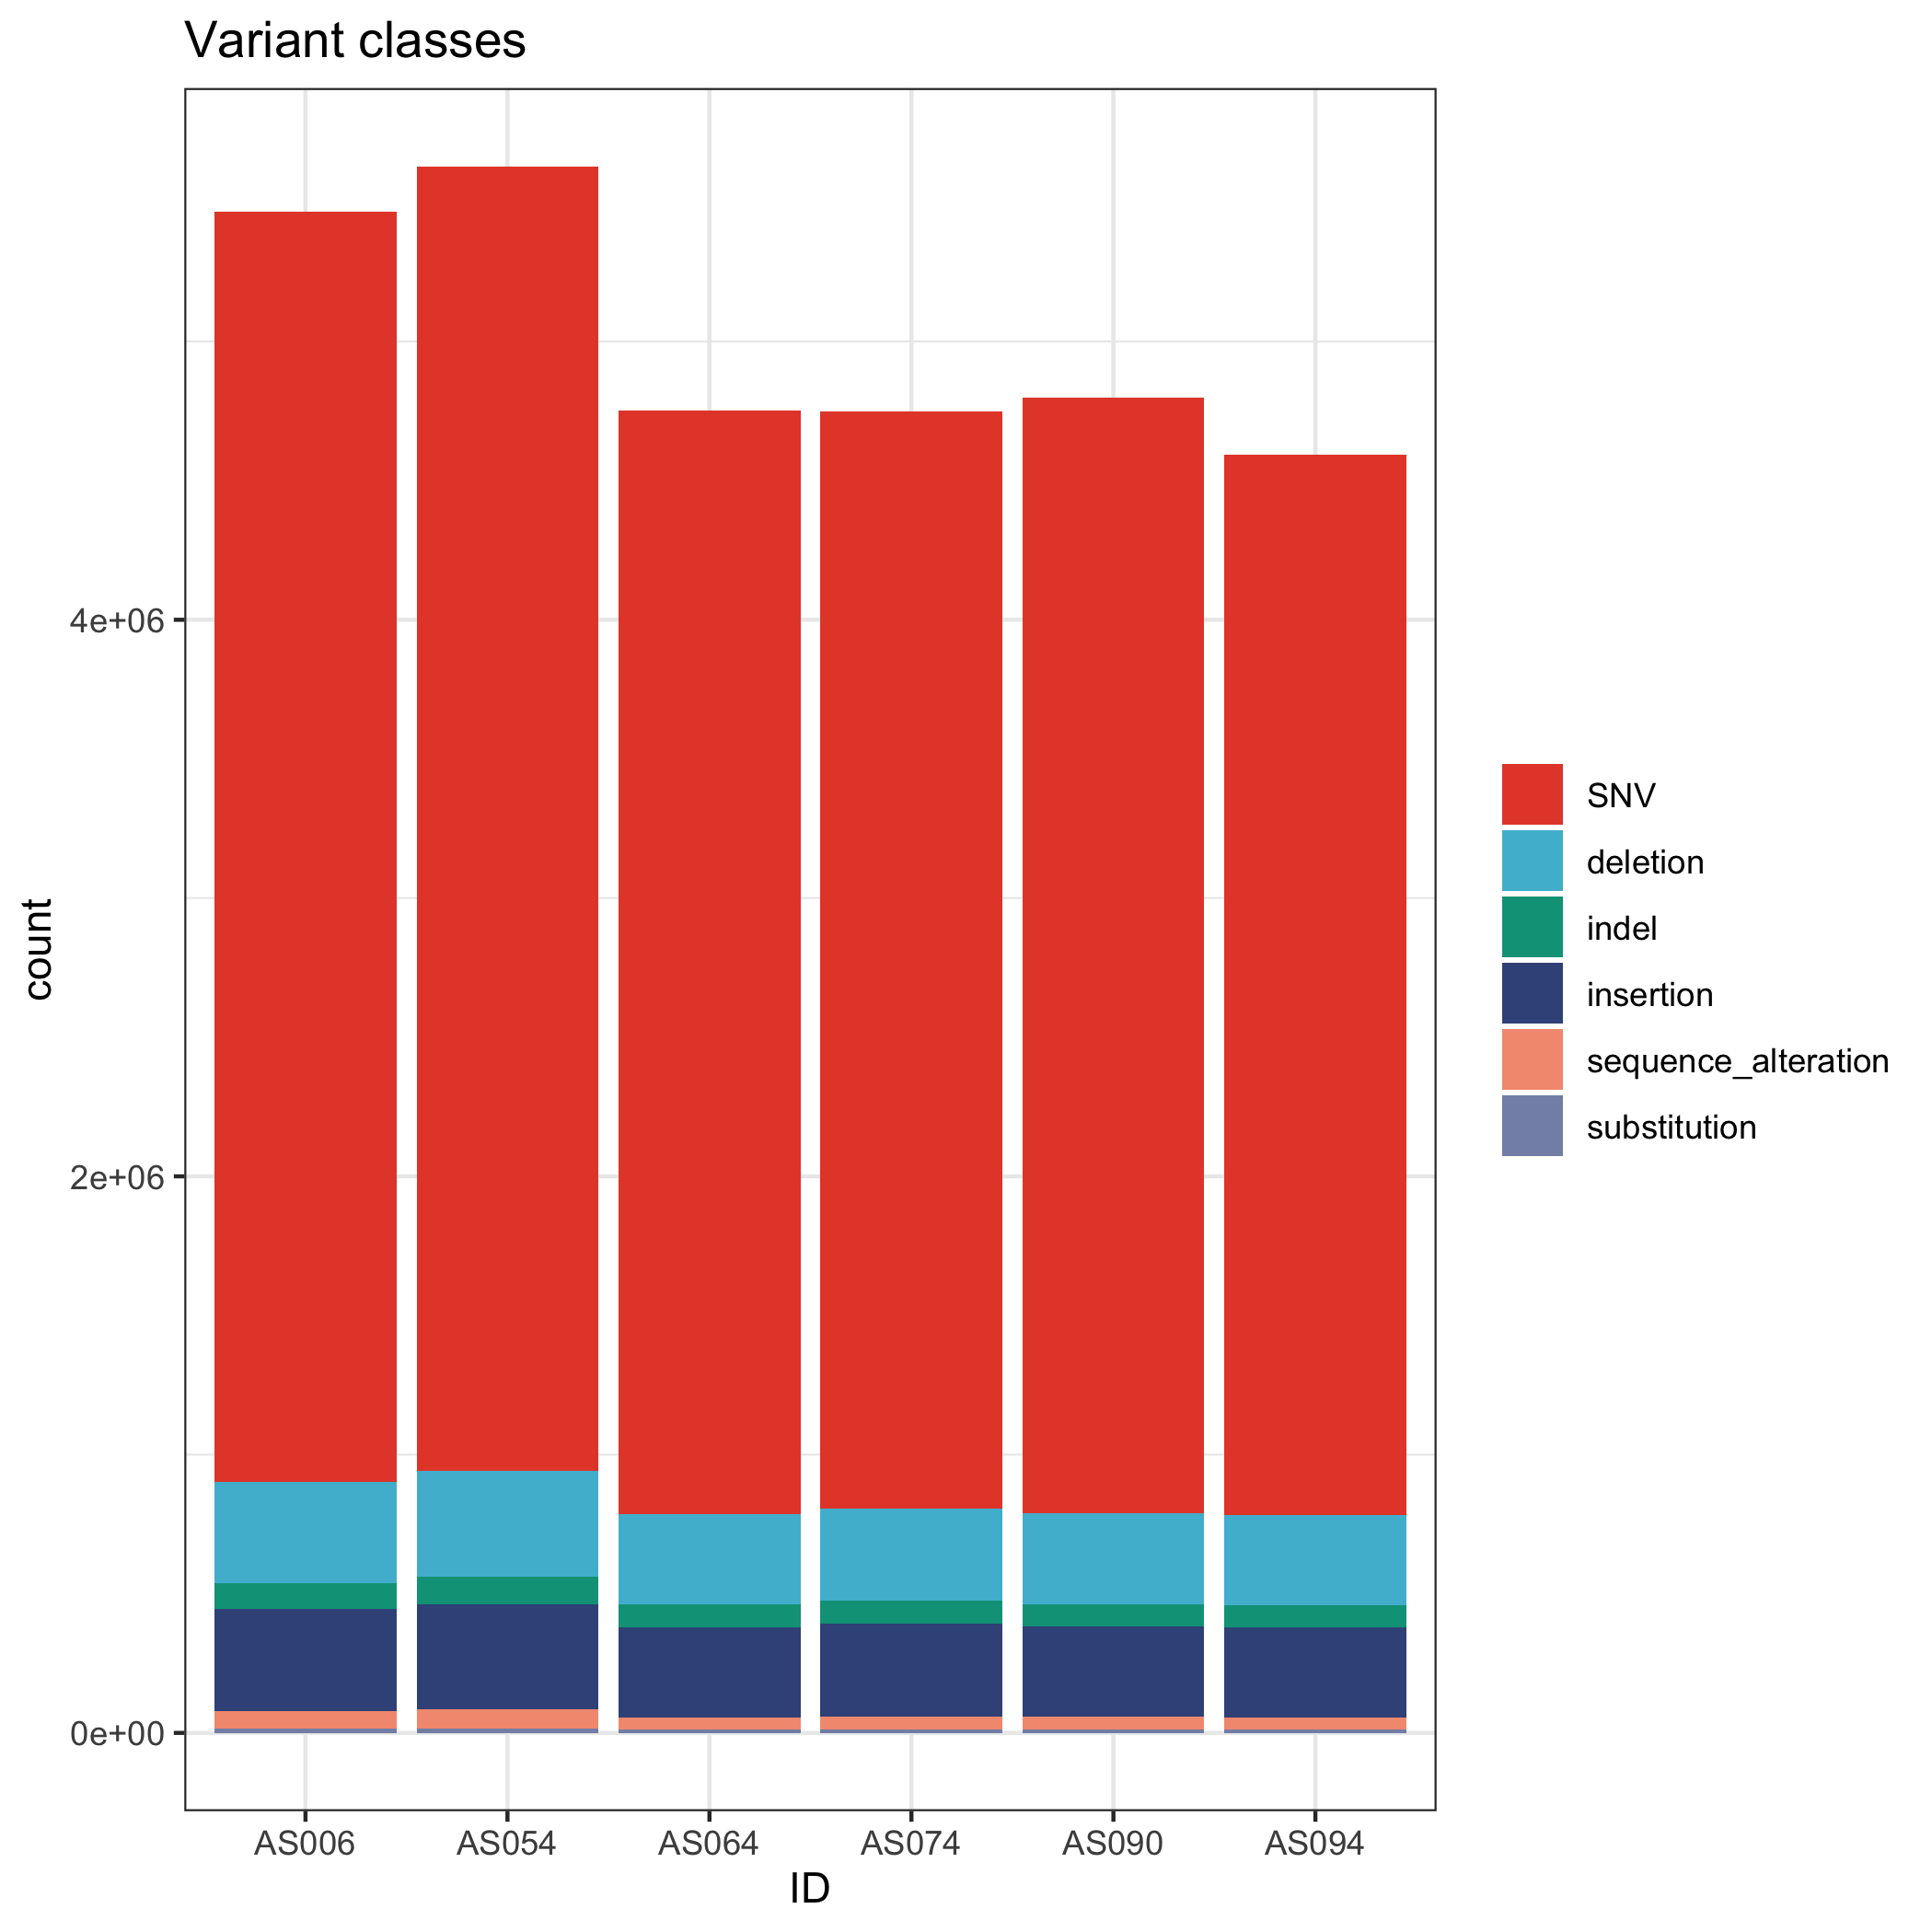
\includegraphics[width=0.8\textwidth]{fig/variantClass.png}
\decoRule
\caption{\textbf{Variant classes among all samples}}
\label{fig:variantClass}
\end{figure}

%%%%%%%%%%%%%%%%%%%%%%%%%%%%%%%%%%%%%%%%%%%%%%%%%%%%%%%%%%%%%%%%%%%%%%%%%%%%%
%  Subsection 
%%%%%%%%%%%%%%%%%%%%%%%%%%%%%%%%%%%%%%%%%%%%%%%%%%%%%%%%%%%%%%%%%%%%%%%%%%%%%

\subsection{Functional annotation of genetic variants}

Once the genetic variants are identified, the following challenge is to understand their functional consequences, i.e.the effect that they produce on the gene and if they cause a specific phenotype. I have used \textsc{variant effect predictor} (\textsc{vep}, \cite{mclaren2016ensembl}) provided by Ensembl (\cite{howe2020ensembl}) to annotate the genetic variant discovered in the six GREP samples. \textsc{vep} is currently the most updated and comprehensive toolset for the analysis, annotation, and prioritization of genomic variants in coding and non-coding regions based on an extensive collection of genomic annotations. \textsc{vep} can determine the effect of variants (SNPs, insertions, deletions, CNVs or structural variants) on genes, transcripts, and protein sequence, as well as regulatory regions.

\begin{comment}
{\small
\begin{sidewaystable}
\caption{Table of Consequences}
\label{tab:csqVEP}
\centering
\begin{adjustbox}{width=1\textwidth}
\begin{tabular}{c c c c}
\toprule
\tabhead{SO term} & \tabhead{SO description} & \tabhead{SO accession} & \tabhead{Impact} \\
\midrule
transcript ablation & A feature ablation whereby the deleted region includes a transcript feature & SO:0001893 & HIGH \\
splice acceptor variant & A splice variant that changes the 2 base region at the 3' end of an intron & SO:0001574 & HIGH \\
splice donor variant & A splice variant that changes the 2 base region at the 5' end of an intron & SO:0001575 & HIGH \\
stop gained & A sequence variant whereby at least one base of a codon is changed, resulting in a premature stop codon, leading to a shortened transcript & SO:0001587 & HIGH \\
frameshift variant & A sequence variant which causes a disruption of the translational reading frame, because the number of nucleotides inserted or deleted is not a multiple of three & SO:0001589 & HIGH \\
stop lost & A sequence variant where at least one base of the terminator codon (stop) is changed, resulting in an elongated transcript & SO:0001578 & HIGH \\
start lost & A codon variant that changes at least one base of the canonical start codon & SO:0002012 & HIGH \\
transcript amplification & A feature amplification of a region containing a transcript & SO:0001889 & HIGH \\
inframe insertion & An inframe non synonymous variant that inserts bases into in the coding sequence & SO:0001821 & MODERATE \\
inframe deletion & An inframe non synonymous variant that deletes bases from the coding sequence & SO:0001822 & MODERATE \\
missense variant & A sequence variant, that changes one or more bases, resulting in a different amino acid sequence but where the length is preserved & SO:0001583 & MODERATE \\
protein altering variant & A sequence variant which is predicted to change the protein encoded in the coding sequence & SO:0001818 & MODERATE \\
splice region variant & A sequence variant in which a change has occurred within the region of the splice site, either within 1-3 bases of the exon or 3-8 bases of the intron & SO:0001630 & LOW \\
incomplete terminal codon variant & A sequence variant where at least one base of the final codon of an incompletely annotated transcript is changed & SO:0001626 & LOW \\
start retained variant & A sequence variant where at least one base in the start codon is changed, but the start remains & SO:0002019 & LOW \\
stop retained variant & A sequence variant where at least one base in the terminator codon is changed, but the terminator remains & SO:0001567 & LOW \\
synonymous variant & A sequence variant where there is no resulting change to the encoded amino acid & SO:0001819 & LOW \\
coding sequence variant & A sequence variant that changes the coding sequence & SO:0001580 & MODIFIER \\
mature miRNA variant & A transcript variant located with the sequence of the mature miRNA & SO:0001620 & MODIFIER \\
5 prime UTR variant & A UTR variant of the 5' UTR & SO:0001623 & MODIFIER \\
3 prime UTR variant & A UTR variant of the 3' UTR & SO:0001624 & MODIFIER \\
non coding transcript exon variant & A sequence variant that changes non-coding exon sequence in a non-coding transcript & SO:0001792 & MODIFIER \\
intron variant & A transcript variant occurring within an intron & SO:0001627 & MODIFIER \\
NMD transcript variant & A variant in a transcript that is the target of NMD & SO:0001621 & MODIFIER \\
non coding transcript variant & A transcript variant of a non coding RNA gene & SO:0001619 & MODIFIER \\
upstream gene variant & A sequence variant located 5' of a gene & SO:0001631 & MODIFIER \\
downstream gene variant & A sequence variant located 3' of a gene & SO:0001632 & MODIFIER \\
TFBS ablation & A feature ablation whereby the deleted region includes a transcription factor binding site & SO:0001895 & MODIFIER \\
TFBS amplification & A feature amplification of a region containing a transcription factor binding site & SO:0001892 & MODIFIER \\
TF binding site variant & A sequence variant located within a transcription factor binding site & SO:0001782 & MODIFIER \\
regulatory region ablation & A feature ablation whereby the deleted region includes a regulatory region & SO:0001894 & MODERATE \\
regulatory region amplification & A feature amplification of a region containing a regulatory region & SO:0001891 & MODIFIER \\
feature elongation & A sequence variant that causes the extension of a genomic feature, with regard to the reference sequence & SO:0001907 & MODIFIER \\
regulatory region variant & A sequence variant located within a regulatory region & SO:0001566 & MODIFIER \\
feature truncation & A sequence variant that causes the reduction of a genomic feature, with regard to the reference sequence & SO:0001906 & MODIFIER \\
intergenic variant & A sequence variant located in the intergenic region, between genes & SO:0001628 & MODIFIER \\
\bottomrule\\
\end{tabular}
\end{adjustbox}
\end{sidewaystable}
}

\end{comment}
Table \ref{tab:csqVEP} (adapted from \cite{mclaren2016ensembl}) describes the classification of the consequences in the Ensembl Variation data base. The impact of the variant on the gene product is classified in four categories: high, moderate, low, and modifier. Examples of variations with high impact are mutations that cause premature termination of the transcription (stop gained) or that suppress transcription (start lost). The classification includes variants in genic (e.g. missense), regulatory (e.g. located in transcription factor binding site) and intergenic regions. In the analysis of the GREP samples we refer to these categories. 

Overall,  TABELLA sample \#high \#moderate \#low \#modifier 

Figure \ref{fig:grid_cons} shows the outcome for the most deleterious variant of \textsc{vep} stratified by categories of impact. Among the variants with high impact ....

%Most of the consequence annotated by VEP are intron variant (49\%), non-coding transcript variant (14.7\%), upstream and downstream gene variant (8.1\% , 8\%) (Figure \ref{fig:vep_AS006_sum_allConsequence}). The count of each Consequence type are reported in Table \ref{tab:AS006_chr1_consequence_count}. 

%Another statistic analysis focused on Coding region show us that the more representative consequence are Synonimous variant (50.8\%) followed by Missence variant (47\%) (Figure \ref{fig:vep_AS006_sum_codingConsequence}). Furthermore VEP provide also a SIFT score that predicts whether an amino acid substitution affects protein function (Figure \ref{fig:vep_AS006_sum_sift}) and POLYPHEN score that predicts possible impact of an amino acid substitution on the structure and function of a human protein using straightforward physical and comparative considerations (Figure \ref{fig:vep_AS006_sum_polyphen}).%Both score are used for a good analysis and we denote 604 deleterious change in the amminoacids only in chromosome 1 of our sample (AS006) (Figure \ref{fig:vep_AS006_sum_sift}).

\begin{comment}
{\small
\begin{table}
\caption{Percentage of each class of impact}
\label{tab:percentageImpact}
\centering
\begin{adjustbox}{width=0.7\textwidth}
\begin{tabular}{1 1 1 1 1 }
\toprule
\tabhead{ID} & \tabhead{HIGH} & \tabhead{MODERATE} & \tabhead{LOW} & \tabhead{MODIFIER} \\
\midrule
 AS006 & 0.022 & 0.254 & 0.345 & 99.4 \\
 AS054 & 0.023 & 0.254 & 0.353 & 99.4 \\
 AS064 & 0.021 & 0.249 & 0.339 & 99.4 \\
 AS074 & 0.022 & 0.252 & 0.342 & 99.4 \\
 AS090 & 0.022 & 0.249 & 0.340 & 99.4 \\
 AS094 & 0.022 & 0.257 & 0.352 & 99.4 \\
\bottomrule\\
\end{tabular}
\end{adjustbox}
\end{table}
}
\end{comment}
\begin{figure}[H]
\centering
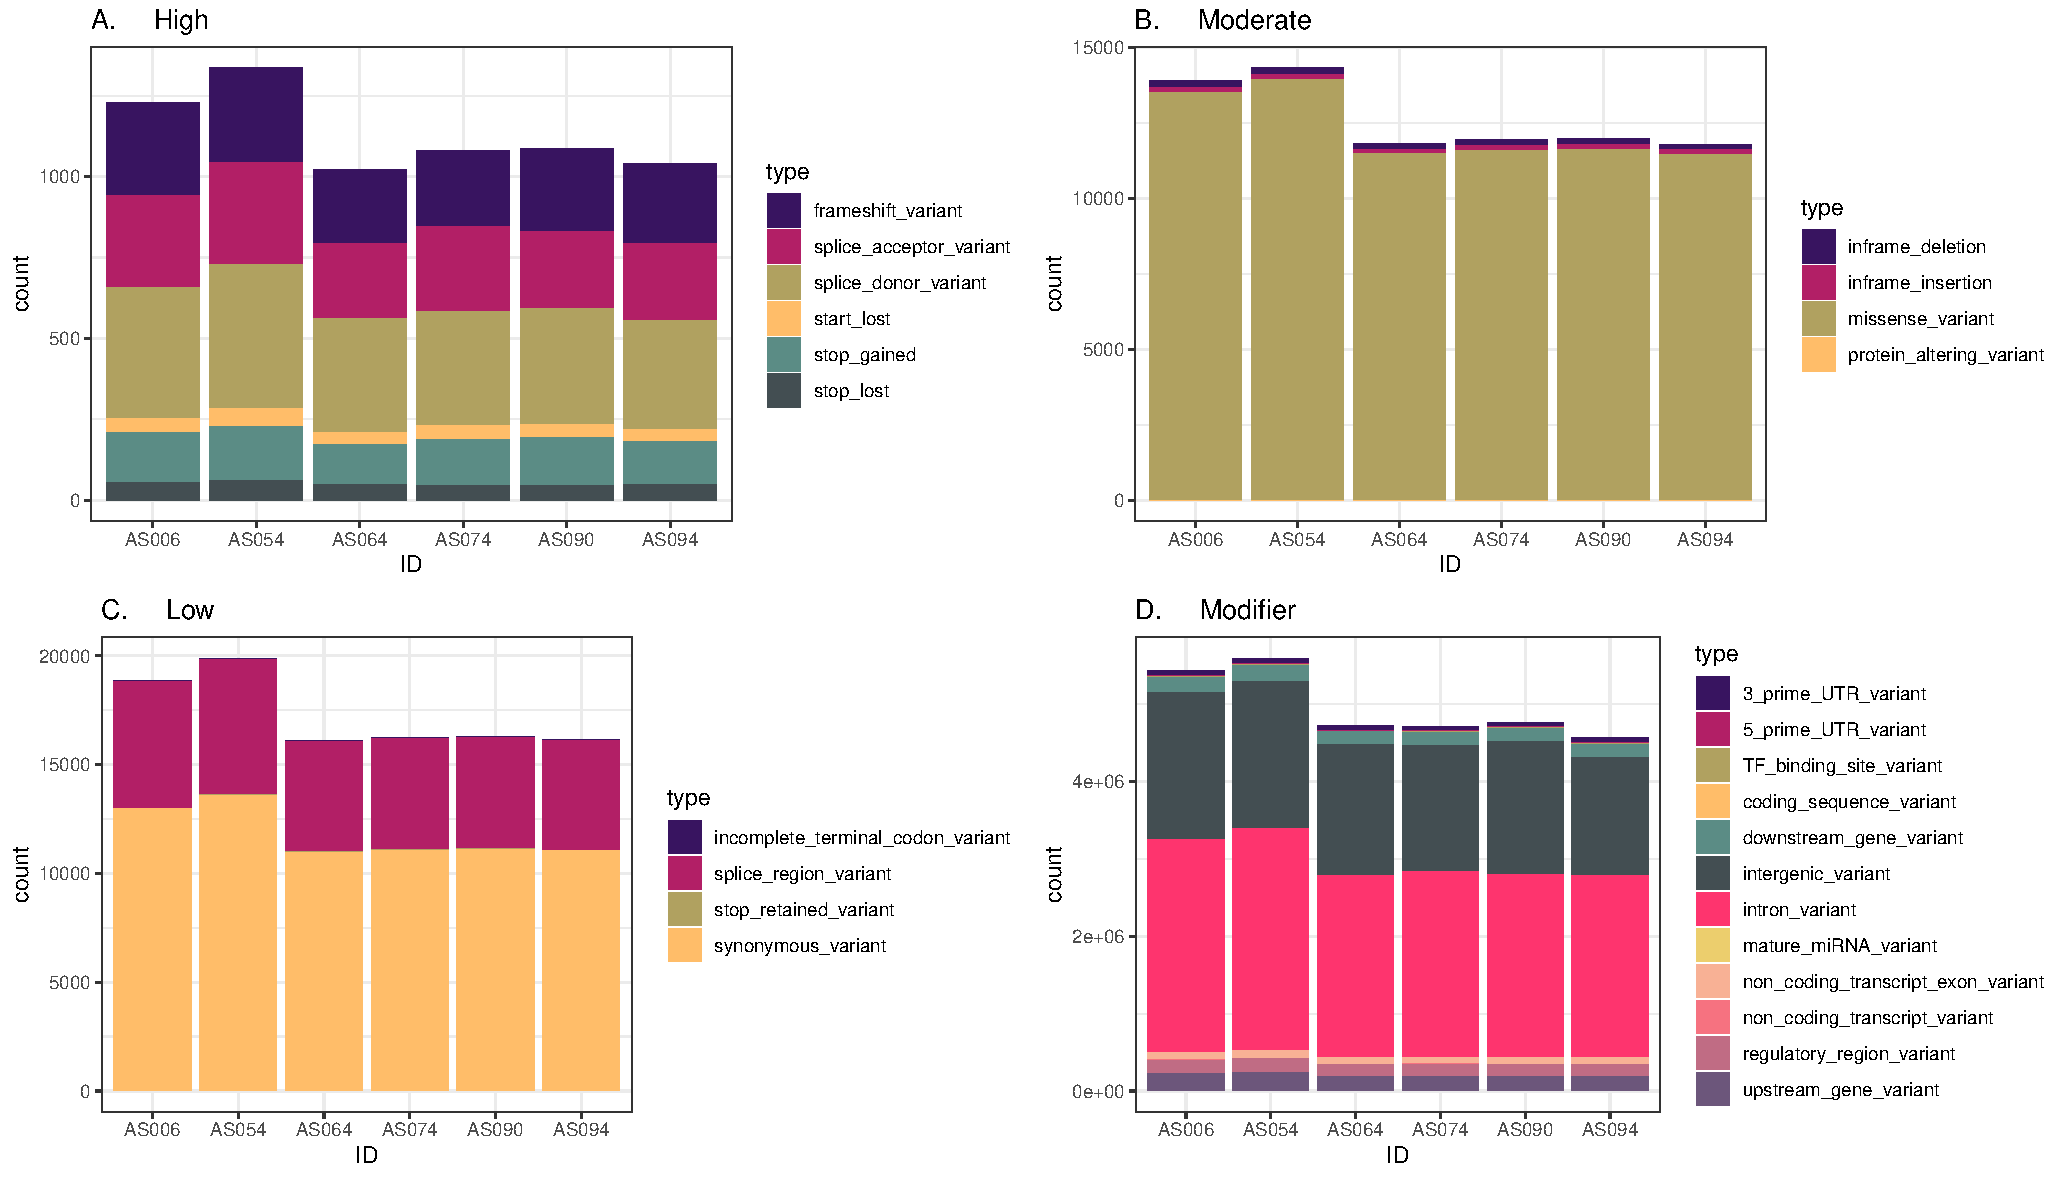
\includegraphics[width=1\textwidth]{fig/grid_cons.pdf}
\decoRule
\caption{\textbf{Fig A High:} XXXX \textbf{Fig B Moderate:} XXX.\textbf{Fig C Low:} XXX.\textbf{Fig D Modifier:} XXX.}
\label{fig:grid_cons}
\end{figure}

%%%%%%%%%%%%%%%%%%%%%%%%%%%%%%%%%%%%%%%%%%%%%%%%%%%%%%%%%%%
%  Subsection 
%%%%%%%%%%%%%%%%%%%%%%%%%%%%%%%%%%%%%%%%%%%%%%%%%%%%%%%%%%%

\subsection{Identification of causative variants }
%Now we want to know what VEP really does with our data. Essentially it adds all informations described before plus more other to our VCF file for each site (Figure \ref{fig:vep_example_output}). 
\subsubsection{Development of a pipeline for variant prioritization}

The rationale behind the identification of genetic variants responsible for PL is based on the hypotheses that the causative variants are likely to be among those classified as detrimental and that more than one mutation can contribute to the phenotype. Furthermore, we assume that the phenotype is a complex trait, i.e. the combination of variants at more than one gene might have caused the miscarriage, therefore we seek for a list of variants in more than one gene or regulatory region, rather than a single variant. Under these assumptions I used the information contained in the variant annotations to search for those more likely to be deleterious and possibly causative.\\

I contributed to develop a pipeline (\url{https://github.com/ezcn/grep}) that analyze genomic variants within individual genome sequences to prioritize those possibly causative. A scheme of how the algorithm works is presents in Figure \ref{fig:scriptPipeline}. The pipeline is optimized for genomic regions containing coding sequences, while the analysis of regulatory regions is under development. In particular, in this first version of the pipeline we use a combination of the following information:  
\begin{itemize}
\item \textbf{Allele that cause the consequence.} We consider the \textbf{count} of the allele, i.e. if the individual has one or two allele, assuming that having two alleles is worst than having only one. We consider \textbf{allele frequency} in the 1000Genomes (\cite{1000genome2015global}) and gnomeAD (\cite{karczewskigenome}) data bases, representing reference population; we assume that if the allele is common than it is less likely to be detrimental. 
\item \textbf{Type and severity of the consequence.} We use the ranking illustrated in Table \ref{tab:csqVEP} to give priorities to consequences with higher impact on the phenotype.  
\item \textbf{pLI score.} pLI is the probability of a gene of being loss-of-function intolerant (\cite{lek2016analysis}). A value of pLI>0.9 suggests that the gene is likely to not tolerate mutations that alter its function, therefore variants located in these genes are more likely to be prioritized.  
\item \textbf{CADD score.} The Combined Annotation Dependent Depletion (CADD) is a  score that integrates multiple annotations into one metric by contrasting variants that survived natural selection with simulated mutations (\cite{kircher2014general}, \cite{rentzsch2019cadd}). The highest the CADD score, the more likely is the pathogenicity of a variant and it applies both to coding and non-coding variants. 
\item \textbf{Genes associated with miscarriages or involved in embryonic development.} We assign high priority to variants located in these sets of genes: 4651 essential  (\cite{blomen2015gene}, \cite{wang2015identification}, \cite{hart2015high}); 3801 lethal (\cite{dawes2019gene}); genes involved in the embyonic development (GO:0009790); genes DDD (\cite{firth2011deciphering}, \cite{firth2009decipher}); a manually curated list of genes that have been associated with miscarriages, obtained from literature (\cite{laisk2019genetic}, \cite{pereza2017systematic}, \cite{qiao2016whole}, \cite{rull2012genetics}, \cite{colley2019potential}, \cite{quintero2017novel}). 
\end{itemize}

The first part of the pipeline works at \textit{per}-individual, \textit{per}-site level producing annotations like those illustrated in Figure \ref{fig:vep_example_output}. Annotations are filtered or ranked in the second part of the pipeline. Overall, the pipeline takes as input the the genetic variants in vcf format and produces a table with sites that pass the filtering or have high rank (Figure \ref{fig:scriptPipeline}).  


%Know what allele produce the consequence is essential for us to understand if our samples are heterozygous or homozygous for that allele.

%In VEP we have a tidy table of Consequences divided into 4 different impacts by severity. For us know the consequence is crucial for attribute value at that site.

%The last two important things are Ensamble gene ID for going back to the gene in that position, and the frequencies are as much important that its allow selecting only these variants that are rare in all population.


\subsubsection{Identification of putatively detrimental variants in the \textit{AHNAK2} gene by raw filtering of annotated variants}

Meanwhile, as a proof of principle, we applied raw filtering based on the combination of several criteria like allele frequencies in the general population (selected to be extremely rare), homozygosity, impact of the allele with consequences. Our preliminary results identify a number of putatively detrimental mutations. Among those, three samples carry two homozygous missense mutations in the \textit{AHNAK2} cancer-related gene, coding a cytoplasmic nucleoprotein whose high expression is associated with negative prognosis of several cancers\cite{}.


%This number is too high to find a causative gene or genetic pathway made up of about 15-30 genes for recurrent miscarriage.
%We need to filter much more and deeper. 

%To do that we have build a bioinformatics software that makes an analysis that is per-individual, per-site and consists of a "Hard Filtering" using a set of parameters that we choose. This software takes in input the file, that is provided after the analysis with VEP software, in VCF format and provides us a table with only sites that pass the filtering.
The criteria with which the first filter was made are the following:

\begin{itemize}
\item Rare variants (allele frequency <1\%)
\item VEP impact Moderate or High 
\item Homozygous for the allele with consequences
\end{itemize}

The resulting after this kind of filtering is that all samples have a low number of candidate sites and their consequence  is only Missence variant (Figure \ref{fig:script_rawFiltering_homzygous}).

\subsubsection{Identification of putatively detrimental variants in the \textit{LAMA5} gene by ranking of annotated variants}

Within genic regions we identified three to ten genetic variants per sample of high (splice-donor) and moderate (missense) impact with frequency lower than 5\% in gnomAD and 1000 Genomes populations, located in twenty-eight genes involved in early embryonic development. Four genes with these variants are involved in the gonadotropin-releasing hormone receptor pathway and two in the integrin signalling pathway. Of particular relevance four samples have multiple hetrozygous missense mutations at four sites in \textit{LAMA5}, a gene that regulates the attachment, migration, and organization of cells into tissues during embryonic development.\\


After this fist attempt we made another filter not by limiting for homozygous variants but by checking if the variant is into a lists of genes important for embryonic development or for the cell cycle. This lists was taken by GENEONTOLOGY (\href{http://geneontology.org/}{GO}), we have searched for a specific category and taken all genes below it.

We have more "candidate" sites and for each site we know if there is in a gene involved in Embryo development (GO:0009790) or in the cell cycle (GO:0007049) or in both (Figure \ref{fig:script_rawFiltering_CellEmbryo}). The type of Consequence is much similar to the previous filter with most of all sites that have a Missence variant (Figure \ref{fig:script_rawFiltering_geneList}), furthermore, the number of sites is on the order that we want and it will be relevant for the future development of this software.

With this lists, we have repeat the first filter and we have seen that the homozygous sites are less enriched then heterozygous sites (Figure \ref{fig:script_rawFiltering_CellEmbryo_homozygous}). 

\begin{figure}[H]
\centering
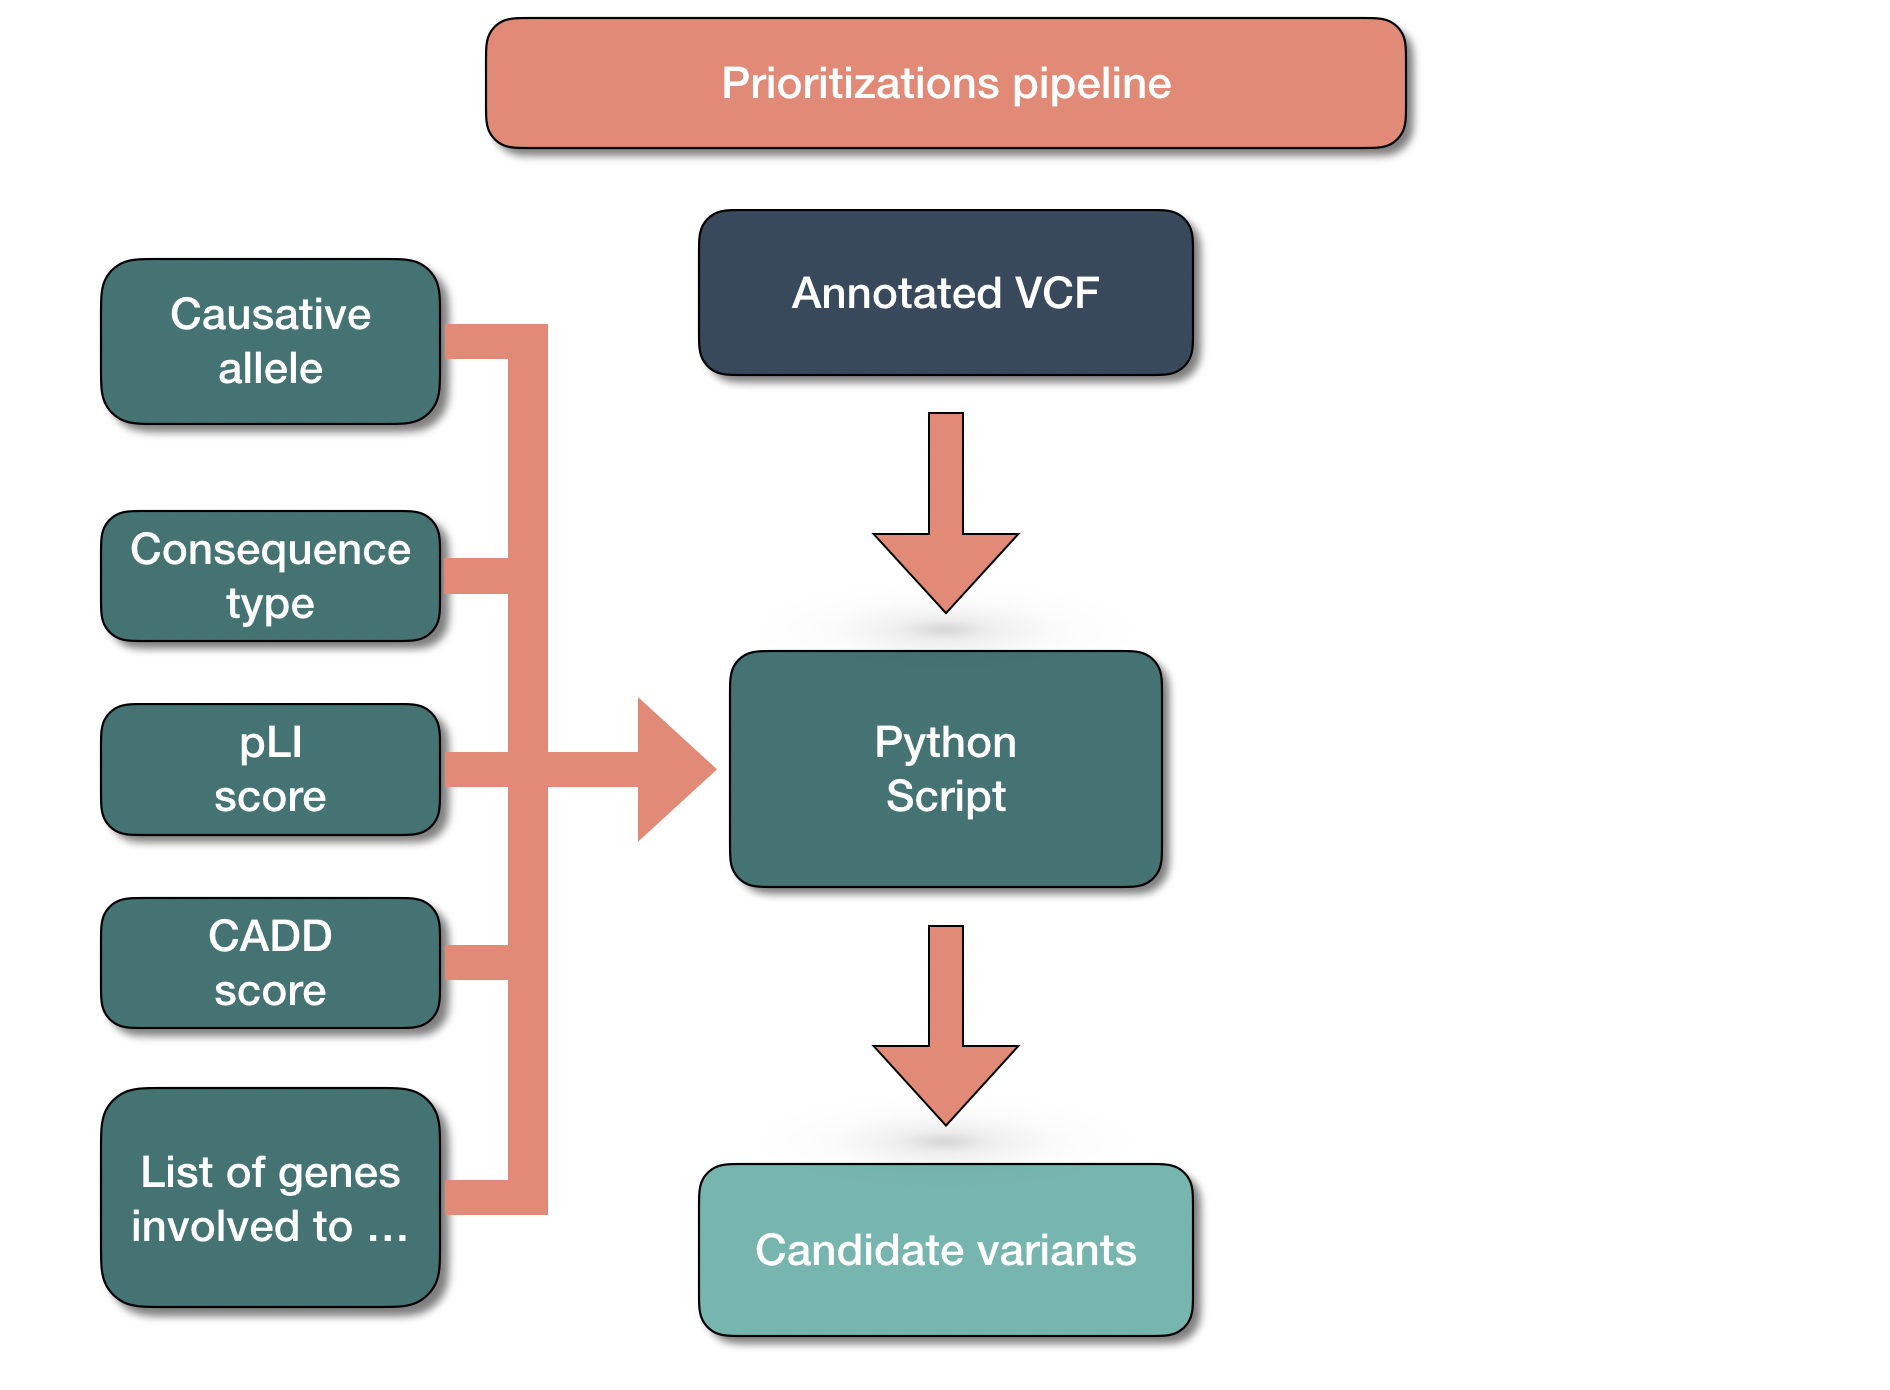
\includegraphics[width=0.85\textwidth]{fig/scriptPipeline.png}
\decoRule
\caption{\textbf{Prioritization pipeline with combined scores and lists of genes.}}
\label{fig:scriptPipeline}
\end{figure}

\begin{figure}[th]
\centering
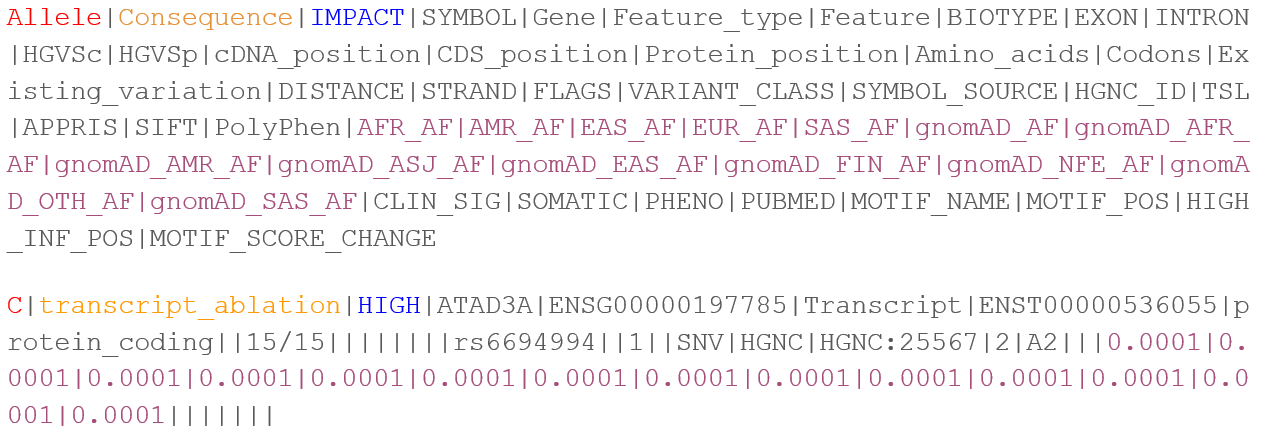
\includegraphics[width=1\textwidth]{fig/vep_example_output.PNG}
\decoRule
\caption[Summary Consequence]{Header and example output of VEP software}
\label{fig:vep_example_output}
\end{figure}


\begin{figure}[H]
\centering
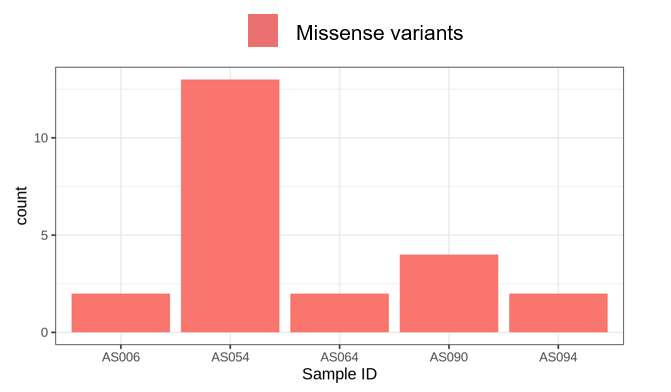
\includegraphics[width=0.85\textwidth]{fig/script_rawFiltering_homozygous.PNG}
\decoRule
\caption[Raw Filtering]{All the sites have only Missence variant.}
\label{fig:script_rawFiltering_homzygous}
\end{figure}

\begin{figure}[H]
\centering
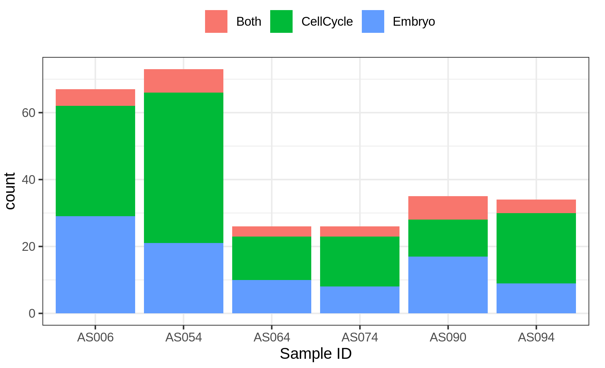
\includegraphics[width=0.85\textwidth]{fig/script_rawFiltering_CellEmbryo.PNG}
\decoRule
\caption[Raw Filtering]{Distribution of consequence after checking in Embryo or/and CellCycle lists.}
\label{fig:script_rawFiltering_CellEmbryo}
\end{figure}

\begin{figure}[H]
\centering
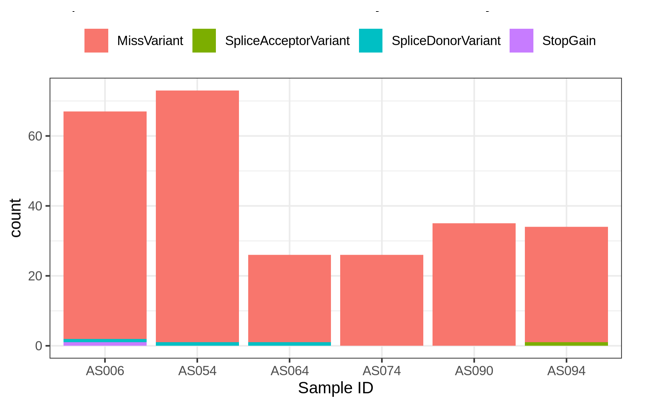
\includegraphics[width=0.75\textwidth]{fig/script_rawFiltering_geneList.PNG}
\decoRule
\caption[Raw Filtering]{Type of Consequence after filtering with gene lists.}
\label{fig:script_rawFiltering_geneList}
\end{figure}

\begin{figure}[H]
\centering
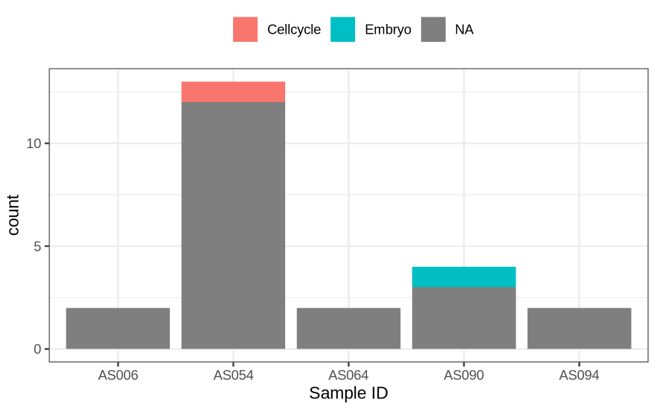
\includegraphics[width=0.75\textwidth]{fig/script_rawFiltering_CellEmbryo_homozygous.png}
\decoRule
\caption[Raw Filtering]{Precence or not in gene lists for samples that are homozygous.}
\label{fig:script_rawFiltering_CellEmbryo_homozygous}
\end{figure}

%%%%%%%%%%%%%%%%%%%%%%%%%%%%%%%%%%%%%%%%%%%%%%%%%%%%%%%%%%%
%  Subsection 
%%%%%%%%%%%%%%%%%%%%%%%%%%%%%%%%%%%%%%%%%%%%%%%%%%%%%%%%%%%

\subsection{Overlapping.}
With the results provided by our software, we have checked if there is an overlapping between samples in the homozygous sites.
In half of the samples, we have overlapping in the same gene and transcript (Table \ref{tab:overlapping}).

Wiht Ensembl transcript we know the gene is \emph{AHNAK2}.
In two of three is the same variant, change of Glutammic acid in Aspartic acid, (supported by Variant ID) the remaining sample has another variant, change of Leucine in Valine, further upstream than the others (Figure \ref{fig:gene_ahnak2}). 
\todo{Nella discussione parlare maggiormente sul perchè l'overlap sia una cosa molto positiva in soli 3 campioni. Parlare anche di cosa si conosce del gene.}
\begin{comment}
{\small
\begin{table}
\caption{Overlapping in three samples}
\label{tab:overlapping}
\centering
\begin{adjustbox}{width=1\textwidth}
\begin{tabular}{c c c c c c c}
\toprule
\tabhead{Sample ID} & \tabhead{Chr} & \tabhead{Position} & \tabhead{Variant ID} & \tabhead{CSQ allele} & \tabhead{CSQ allele count} & \tabhead{Transcript}\\
\midrule
AS054 & chr14 & 104944965 & rs200535803-COSM2026918 & C & 2 & ENST00000333244\\
AS074 & chr14 & 104952007 & rs55791176 & G & 2 & ENST00000333244\\
AS064 & chr14 & 104952007 & rs55791176 & G & 2 & ENST00000333244\\
\bottomrule\\
\end{tabular}
\end{adjustbox}
\end{table}
}
\end{comment}


\begin{figure}[th]
\centering

\includegraphics[width=1\textwidth]{fig/gene_ahnak2.png}
\decoRule
\caption[Gene]{\emph{AHNAK2} overlapping transcripts (below).}
\label{fig:gene_ahnak2}
\end{figure}

%%%%%%%%%%%%%%%%%%%%%%%%%%%%%%%%%%%%%%%%%%%%%%%%%%%%%%%%%%%%%%%%%%%%%%%%%%%%%%%



%%%%%%%%%%%%%%%%%%%%%%%%%%%%%%%%%%%%%%%%%%%%%%%%%%%%%%%%%%%%%%%%%%%%%%%%%%%%%%%

\chapter{Conclusions and Future Perspectives(3-6 pagine)}





\chapter{Materials and Methods(5-10 pagine)}

\section{Explore little graph and detection bubble}  Depth first traversal or Depth first Search is a recursive algorithm for searching all the vertices of a graph or tree data structure. The purpose of the algorithm is to mark each vertex as visited while avoiding cycles.

The DFS algorithm works as follows:

-Start by putting any one of the graph's vertices on top of a stack.
-Take the top item of the stack and add it to the visited list.
-Create a list of that vertex's adjacent nodes. Add the ones which aren't in the visited list to the top of stack.
-Keep repeating steps 2 and 3 until the stack is empty.
\\ 

\begin{verbatim}

def dfs(graph, start, visited=None):
    if visited is None:
        visited = set()
    visited.add(start)
    print(start)
    for next in graph[start] - visited:
        dfs(graph, next, visited)
    return visited

graph = {'0': set(['1', '2']),
         '1': set(['0', '3', '4']),
         '2': set(['0']),
         '3': set(['1']),
         '4': set(['2', '3'])}

dfs(graph, '0')
\end{verbatim}

Breadth first traversal or Breadth first Search is a recursive algorithm for searching all the vertices of a graph or tree data structure.
he algorithm works as follows:

-Start by putting any one of the graph's vertices at the back of a queue.
-Take the front item of the queue and add it to the visited list.
-Create a list of that vertex's adjacent nodes. Add the ones which aren't in the visited list to the back of the queue.
-Keep repeating steps 2 and 3 until the queue is empty.

\begin{verbatim}
def bfs(graph, root): 
    visited, queue = set(), collections.deque([root])
    visited.add(root)
    while queue: 
        vertex = queue.popleft()
        for neighbour in graph[vertex]: 
            if neighbour not in visited: 
                visited.add(neighbour) 
                queue.append(neighbour) 
                
if __name__ == '__main__':
    graph = {0: [1, 2], 1: [2], 2: [3], 3: [1,2]} 
    breadth_first_search(graph, 0)
    
\end{verbatim}

 I implement this code that is availabe on the git repository of the project (\url{https://github.com/ezcn/grep}) 
 
 https://www.programiz.com/dsa/graph-bfs  (guardare qui)
 

\section{Explore large graph }

For this part I use a library of Python.\\ 

Odgi representing large genomic variation graphs with minimal memory overhead requires a careful encoding of the graph entities.
Odgi is based on a node-centric encoding of the graph that is designed to improve
cache coherency when traversing or modifying the graph. This encoding is split
between graph topology and paths, which was found to be important to yielding
a good balance of runtime performance and memory usage on real-world graphs
with large path sets. Each node’s its sequence and inbound and outbound edges
are encoded in a byte array using a variable-length integer encoding scheme.
Edges are described in terms of a relative offset between the rank of this node
in the sorted array of nodes of the graph and the node to which the edge arrives
(or from which it emanates). The set of steps traversing each node is recorded
in a second dynamic integer vector of fixed width entries, compressed so that
only largest integer entry is stored at full width. Each step links a path
identifier, relative ranks of the previous and successive node traversals on the
path, and the rank of the next or previous step among the path steps recorded
at that node. \cite{garrison2020}

Given a graph in GFA format(vedere come inserire il formato e mettere il link), we can build the odgi format using odgi build.

\begin{verbatim}

odgi build -g lil.gfa -o lil.odgi
PYTHONPATH=~/odgi/lib python3

Now we can load the graph and check how big it is:

import odgi

g = odgi.graph() # instatiate a graph
g.load('file.odgi')

\end{verbatim}


For convert GFA format in VCF the code is availabe on the git repository of the project (\url{https://github.com/ezcn/grep}) 

\section {Whole-genome sequence analyses}

\subsection{Sequencing}
Sequencing was done through a service provider (Macrogen s.r.l). In particular, libraries for sequencing were prepared using the Illumina TruSeq DNA PCR-free Library (insert size 350bp) and samples were sequenced at 30X mapped (~110Gb) 150bp PE on HiSeqX. Data were released in as fastq files. 

\subsection{Alignment with reference.} Reads in the fastq file were aligned against the reference genome GRChg38.p12 (\cite{rosenbloom2015ucsc}) using \textsc{bwa} and \textsc{samtools}. \textsc{bwa} (\url{https://github.com/lh3/bwa}) "is a software package for mapping low-divergent sequences against a large reference genome, such as the human genome." Of the three algorithms available in \textsc{bwa} we used \textsc{bwa-mem}  that is generally recommended to analyze 70-100bp Illumina reads. 

For each sample, the following command line takes in input fastq file (paired-end) and gives as output a raw-bam file. 

\begin{verbatim}
~/bin/bwa mem -t 16 -R "@RG\tID:$idsample\tSM:$idsample" \
/mpbastudies3/IMMA/hg38/hg38.p12.fa \ 
/mpbastudies3/181113_Vincenza-Colonna/$namedir/$nameflgz1 \ 
/mpbastudies3/181113_Vincenza-Colonna/$namedir/$nameflgz2 | \ 
/mpba0/mpba-sw/samtools view -b - > \
/mpbastudies3/IMMA/samples/$idsample.raw.bam
\end{verbatim}




\begin{itemize}
\item BWA 
\item SAMTOOLS
\item SAMBAMBA
\item TABIX
\item BGZIP
\item FREEBAYES
\item script in-house github  <-----
\item VEP
\item array-CGH (?)
\item quantitative PCR (?)
\item python (???)
\item R (???)
\end{itemize}




\textsc{samtools} (\url{https://github.com/samtools/samtools}) is a set of utilities for interacting with and post-processing short DNA sequence read alignments in the SAM (Sequence Alignment/Map), BAM (Binary Alignment/Map) and CRAM formats (\href{https://en.wikipedia.org/wiki/SAMtools}{wiki}). 
We have used this software downstream \textsc{bwa-mem} for obtain the BAM from fastq. 

\textbf{Remove PCR duplicate.} During PCR the machine introduces a several PCR duplicate in our sequence, for remove them we have used SAMbamba.

SAMbamba (\url{https://github.com/biod/sambamba}) is a high performance highly parallel robust and fast tool (and library), written in the D programming language, for working with SAM and BAM files.Current functionality is an important subset of samtools functionality, including view, index, sort, markdup, and depth (\href{https://github.com/biod/sambamba#introduction}{git}).We have used the function markdup to remove PCR duplicates. 

\begin{verbatim}
~/bin/sambamba markdup -t 8 -p  \
--tmpdir /scratch --overflow-list-size 500000 \
/mpbastudies3/IMMA/samples/${idflrbam}.raw.sorted.bam \
/mpbastudies3/IMMA/samples/${idflrbam}.bam    
\end{verbatim}

The command line takes in input a raw version of the BAM file for each sample and gives us as output the BAM file without PCR duplicates. 

\textbf{VariantCalling.} Is the process that allows us to identifies sites that differ from the reference for each sample. We have choose FREEBAYES (\url{https://github.com/ekg/freebayes}) that is a Bayesian genetic variant detector designed to find small polymorphisms, specifically SNPs (single-nucleotide polymorphisms), indels (insertions and deletions), MNPs (multi-nucleotide polymorphisms), and complex events (composite insertion and substitution events) smaller than the length of a short-read sequencing alignment (\href{https://github.com/ekg/freebayes}{git}).

\begin{verbatim}
~/bin/freebayes -f /mpbastudies3/IMMA/hg38/hg38.p12.fa \ 
-r ${chr} --gvcf -g 2000  /mpbastudies3/IMMA/samples/${idsample}.bam 
\end{verbatim}

For use this command line is necessary the reference genome (hg38.p12) in fasta format and a BAM for each sample. Furthermore is possible for speedup the process do independent analysis for each chromosome. 

\textbf{Compress and indexing.} When a file was generated is necessary do a compressing and indexing for each one. 

Bgzip (\url{https://www.htslib.org/doc/bgzip.html#DESCRIPTION}) compresses files into a series of small (less than 64K) 'BGZF' blocks. This allows indexes to be built against the compressed file and used to retrieve portions of the data without having to decompress the entire file (\href{https://www.htslib.org/doc/bgzip.html#DESCRIPTION}{wiki}).  

\begin{verbatim}
~/bin/bgzip /mpbastudies3/IMMA/samples/vcf/${idsample}.vcf > \
/mpbastudies3/IMMA/samples/vcf/${idsample}.vcf.gz
\end{verbatim}

The command line take in input the output (VCF) from variant calling and give us the compressed file.  

Tabix (\url{https://www.htslib.org/doc/tabix.html}) indexes a TAB-delimited genome position file in.tab.bgz and creates an index file.

\begin{verbatim}
~/bin/tabix -p vcf /mpbastudies3/IMMA/samples/vcf/${id}.${chr}.vcf.gz 
\end{verbatim}

The command line take in input the compressed file from BGZIP and give the indexed one.

\textbf{Variant Effect Predictor.}  VEP (\url{https://grch37.ensembl.org/info/docs/tools/vep/index.html}) determines the effect of your variants (SNPs, insertions, deletions, CNVs or structural variants) on genes, transcripts, and protein sequence, as well as regulatory regions.
Simply input the coordinates of your variants and the nucleotide changes to find out the:
\begin{itemize}
    \item Alleles, Genes and Transcripts affected by the variants
    \item Location of the variants (e.g. upstream of a transcript, in coding sequence, in non-coding RNA, in regulatory regions)
    \item Consequence of your variants on the protein sequence (e.g. stop gained, missense, stop lost, frameshift)
    \item Known variants that match yours, and associated minor allele frequencies from the 1000 Genomes Project
    \item  SIFT and PolyPhen-2 scores for changes to protein sequence
\end{itemize}


In our case, we have used the command-line version (v96.3) with chosen parameters reported in the command line.

\begin{verbatim}
singularity run -B /mpbastudies3/IMMA/samples/:/data \
/mpba0/mpba-sw/biocontainers/vep-96.3.img \
--af_1kg --af_gnomad --appris --biotype \
--buffer_size 5000 --check_existing --distance 5000 \
--fork 4 --polyphen b --pubmed --regulatory --sift b \
--species homo_sapiens --symbol --tsl --cache \
--dir_cache /mpba0/vcolonna/vepcache/ --offline \
--vcf --variant_class -i /data/vcfconcat/${id}.fullVcf \
-o /data/vepVCF/${id}.fullvep
\end{verbatim}

This software takes in input a final version of the VCF (filtered) and gives to us an annotated version with all the parameters written in the command-line. 

\textbf{}


\printglossary

\printbibliography[heading=bibintoc]


\begin{acknowledgements}
\addchaptertocentry{\acknowledgementname}
\end{acknowledgements}







\end{document}


